\documentclass[class=article, crop=false, 12pt]{standalone}
\usepackage[subpreambles=true]{standalone}
\usepackage{../.common/common}
\allowdisplaybreaks % equation environment from amsmath can break equation between page

\author{Tony Shing}
%\pretitle{Supplementary}

\topic{Note 07 (Mechanics)}
\title{Wave Equation}

\version{2025} % leave blank for omitting

\begin{document}

\maketitle


\begin{overview}

    \begin{center}
        \red{\bf{\ul{The wave equation is a partial differential equation}}}
        \aleq{
            \pdvv[2]{x}y(x,t) = \inv{v^2}\pdvv[2]{t}y(x,t)
        }
        is an equation of $y(x,t)$ -  
        the wave's magnitude as a function of position $x$ and time $t$.\\
        We are going to derive and study its solutions.
    \end{center}

    \begin{itemize}
        \item Derive wave equation - transverse and longitudinal wave
        \item Initial value problem \it{\scriptsize (Not so important)}
        \item Boundary value problem - \cul[red]{What are "Modes" of standing wave}
        \it{\red{\scriptsize (Main focus)}}
    \end{itemize}
\end{overview}



% content begins here
% Section %%%%%%%%%%%%%%%%%%%%%%%%%%%%%%%%%%%%%%%%%%%%%%%%%%%%
\section{Model of Transverse Wave}

We usually use an elastic string to visualize transverse wave travel.

\begin{itemize}
    \item When the string lies flat - Each string segment has a width $\Delta x$.
    
    \begin{center}
        \begin{minipage}{0.4\linewidth}
            \centering
            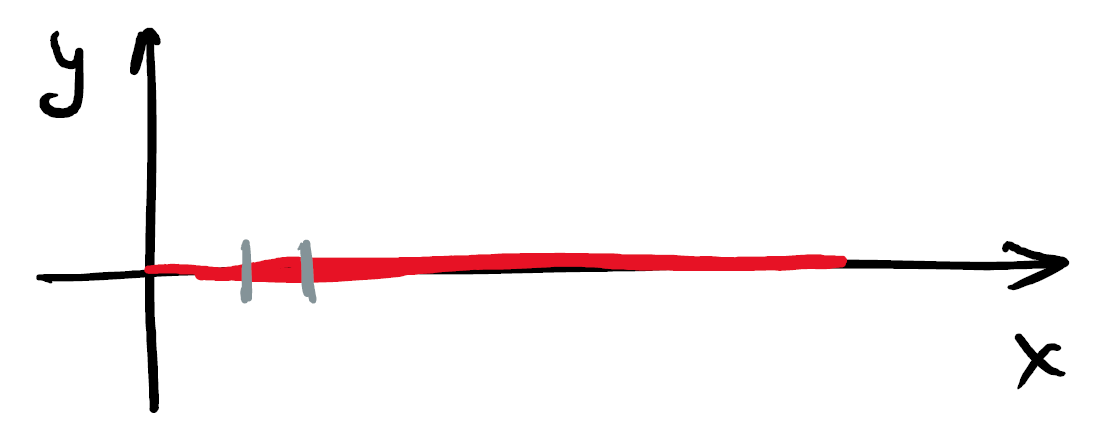
\includegraphics[width=\textwidth]{tran1}
        \end{minipage}
        \hspace{0.05\textwidth}
        $\Rightarrow$
        \hspace{0.05\textwidth}
        \begin{minipage}{0.15\linewidth}
            \centering
            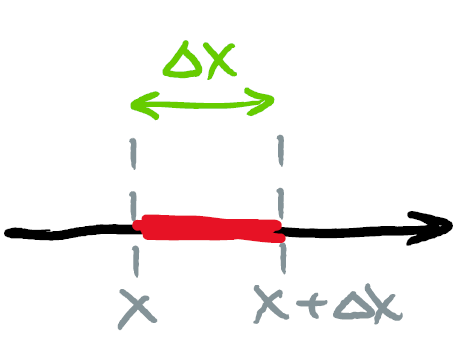
\includegraphics[width=\textwidth]{tran2}
        \end{minipage}
    \end{center}

    \item When the string shakes - The segment jumps up and down,
    horizontal length remains the same, but gain a vertial length.
    
    \begin{center}
        \begin{minipage}{0.4\linewidth}
            \centering
            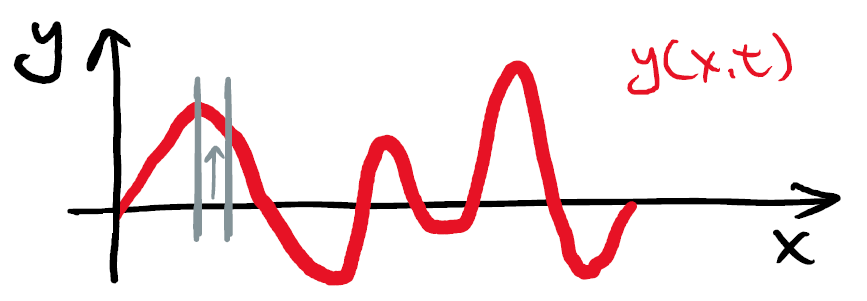
\includegraphics[width=\textwidth]{tran3}
        \end{minipage}
        \hspace{0.05\textwidth}
        $\Rightarrow$
        \hspace{0.05\textwidth}
        \begin{minipage}{0.15\linewidth}
            \centering
            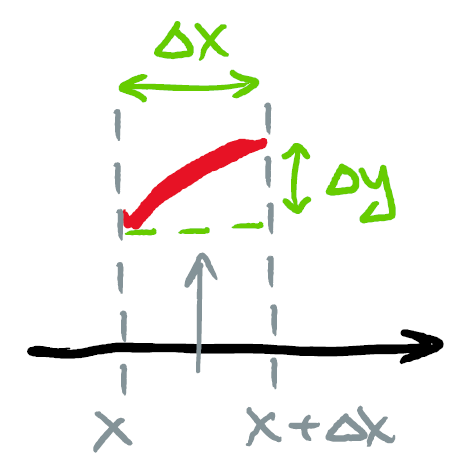
\includegraphics[width=\textwidth]{tran4}
        \end{minipage}
    \end{center}
\end{itemize}

Transverse wave is \red{height of string segments} at different position / time,
which is described by the function $y(x,t)$.\\

\newpage
\bf{\ul{Deriving wave eqauation}}

    \begin{minipage}{0.55\linewidth}
        \begin{enumerate}
            \item \bf{\ul{Equations of forces by Newton's \nth{2} Law}}
            \vskip 1em
            Tension \blue{$\vvec{F}$} must be a function of $x$ because 
            it must be different everywhere along the string.
        \end{enumerate}
    \end{minipage}
    \hspace{0.02\textwidth}\hfill
    \begin{minipage}{0.4\linewidth}
        \centering
        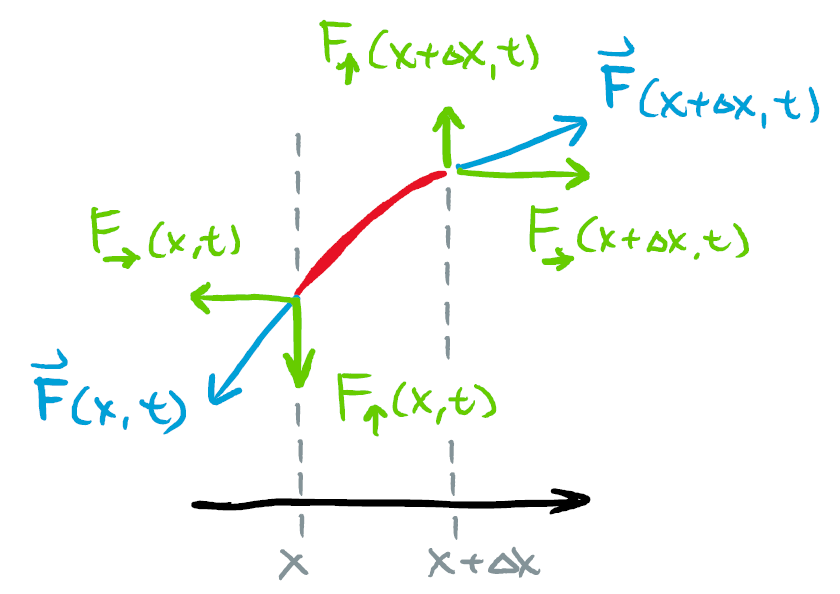
\includegraphics[width=0.9\textwidth]{tran_force}
    \end{minipage}
    
    \vskip 1ex
    \begin{itemize}
        \item[] Separate the tensions' components and write Newton's \nth{2} law in both directions:
        \aleq{
            \bcase{
                \rightarrow : &\quad F_\rightarrow(x+\Delta x,t) - F_\rightarrow(x,t) = \tkn{horzT0}{\cul[red]{0}} \\[1ex]
                \uparrow : &\quad F_\uparrow(x+\Delta x, t) - F_\uparrow(x,t) = (\tkn{mu}{\cul[blue]{\mu}}\Delta x) a_\uparrow
            }
        }
        \addArrow[red]{horzT0}{(10ex,0)}{\scriptsize Horizontal acceleration = 0\\[-1ex]\scriptsize because the string segment\\[-1ex]\scriptsize only jump up \& down}
        {(1.5ex,0.5ex)}{(8ex,0)}
        \addArrow[blue]{mu}{(0,-3ex)}{\scriptsize $\mu = $ Density per unit length\\[-1ex]\scriptsize $\Rightarrow \mu\Delta x = $ Mass of the string segment}
        {(0,-1.5ex)}{(0,-1ex)}

        \hfill\\[1em]
        \bf{\ul{Note}}: There must be no gravity, or else the \nth{2} law becomes
        \aleq{
            F_\uparrow(x+\Delta x, t) - F_\uparrow(x,t) - \cus[blue]{(\mu \Delta x)g}{\text{Extra term}}= (\mu \Delta x) a_\uparrow
        }
        \phantom{\bf{\ul{Note}}:} which will not give us the result of wave equation.
    \end{itemize}


    \vskip 1em
    \begin{minipage}{0.55\linewidth}
        \begin{enumerate}
            \item[2.] \bf{\ul{Analysis by the string's geometry}}
            \vskip 1em
            Tension \blue{$\vvec{F}$} must be parallel to the slope 
            at the 2 end points of the segment. 
            (Otherwise it cannot be tension.)
            
            Meanwhile the slope of the graph $=\pdvv{x}y(x,t)$.
        \end{enumerate}
    \end{minipage}
    \hspace{0.02\textwidth}\hfill
    \begin{minipage}{0.4\linewidth}
        \centering
        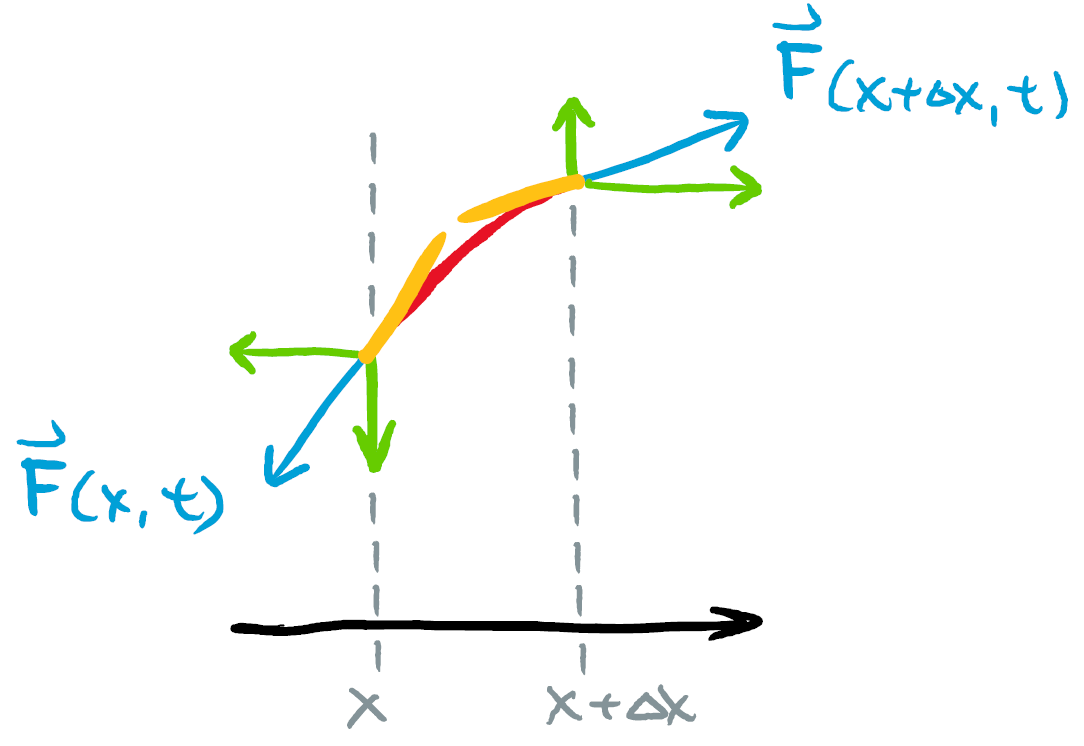
\includegraphics[width=0.9\textwidth]{tran_geom}
    \end{minipage}

    \vskip 2em
    \begin{itemize}
        \item[] Observe that the inclination of tension $\vvec{F}$ can be calculated by $\dfrac{F_\uparrow}{F_\rightarrow}$,
        \aleq{
            \Rightarrow \text{ Relation at end points : } \bcase{
                \frac{F_\uparrow(x+\Delta x, t)}{F_\rightarrow(x+\Delta x, t)} &= \pdvv{x}y(x,t)\eval_{\text{at }x+\Delta x}\\[1em]
                \frac{F_\uparrow(x, t)}{F_\rightarrow(x, t)} &= \pdvv{x}y(x,t)\eval_{\text{at }x}\\
            }
        }
    \end{itemize}
    
\newpage
\begin{enumerate}
    \item[3.] Substitute the above into the Newton's \nth{2} law in vertical direction:
    \addArrow[green]{Fleftright}{(4ex,9.5ex)}
    {\scriptsize Can be grouped together\\[-1ex]\scriptsize because they are equal.\\[-1ex]\scriptsize This is from the Newton's \nth{2} Law\\[-1ex]\scriptsize for horizontal direction}
    {(-0.5ex,3ex)}{(-18ex,-6ex)}
    \addArrow[green]{Fleftright}{(50ex,9.5ex)}{}
    {(0.5ex,3ex)}
    \addArrow[red]{dt2y}{(5ex,8ex)}
    {\scriptsize Vertical acceleration\\[-1ex]\scriptsize = \nth{2} derivative of \\[-1ex]\scriptsize segment's height over $t$}
    {(0,3ex)}{(-14ex,-3ex)}
    \addBentArrow*[blue]{dx2y}{(12.5ex,6ex)}
    {\scriptsize This is just the derivative $\frac{f(x+\Delta x)-f(x)}{\Delta x}$\\[-1ex]\scriptsize $\Rightarrow$ become \nth{2} derivative over $x$}
    {(6ex,0.5ex)}{(12ex,-5ex)}
    \aleq{
        (\mu\Delta x)a_\uparrow &= F_\uparrow(x+\Delta x, t) - F_\uparrow(x,t)\\
        %
        &= \cul[green]{F_\rightarrow(x+\Delta x, t)}\qty[\pdvv{x}y(x,t)\eval_{\text{at }x+\Delta x}] 
            - \cul[green]{F_\rightarrow(x,t)}\qty[\pdvv{x}y(x,t)\eval_{\text{at }x}]\\[2em]
        %
        &= \tkn{Fleftright}{\cul[green]{F_\leftrightarrow}}\qty[\pdvv{x}y(x,t)\eval_{\text{at }x+\Delta x} 
            - \pdvv{x}y(x,t)\eval_{\text{at }x}]\\[1em]
        %
        \mu \cul[red]{a_\uparrow} 
        &= {F_\leftrightarrow} \ \cub[blue]{\frac{\eval{\pdvv{x}y(x,t)}_{\cbox[blue]{\scriptstyle \text{at }x+\Delta x}} 
            - \eval{\pdvv{x}y(x,t)}_{\cbox[blue]{\scriptstyle \text{at }x}}}{\cbox[blue]{\Delta x}}}{}\\
        %
        \mu\tkn{dt2y}{\cul[red]{\pdvv[2]{t}y(x,t)}} &= F_\leftrightarrow \tkn{dx2y}{\cul[blue]{\pdvv[2]{x}y(x,t)}}\\[1em]
        %
        \Aboxed{
            \frac{\mu}{F_\leftrightarrow} \pdvv[2]{t}y(x,t) &= \pdvv[2]{x}y(x,t)
        }
    }
    

\end{enumerate}

Compare with the general form of wave equation $\dinv{v^2}\pdvv[2]{t}y(x,t) = \pdvv[2]{x}y(x,t)$,
we can identify the wave speed of transverse wave as 
\aleq{
    v=\sqrt{\frac{F_\leftrightarrow}{\mu}} = \sqrt{\frac{\text{Horizontal Tension}}{\text{Mass per Length}}}
}


\linesep
\newpage
% Section %%%%%%%%%%%%%%%%%%%%%%%%%%%%%%%%%%%%%%%%%%%%%%%%%%%%
\section{Model of Longitudinal Wave}

We usually use a slinky to visualize longitudinal wave travel.

\begin{itemize}
    \item When the slinky is static - Each peak are of equal spacing.
    
    \begin{center}
        \begin{minipage}{0.45\linewidth}
            \centering
            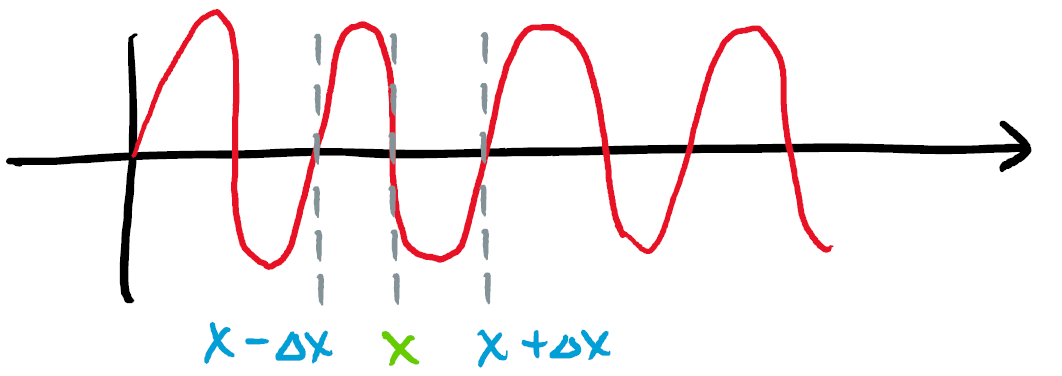
\includegraphics[width=\textwidth]{long1}
        \end{minipage}
    \end{center}

    \item When the slinky shakes - the peaks become unevenly distributed.
    
    \begin{center}
        \begin{minipage}{0.58\linewidth}
            \centering
            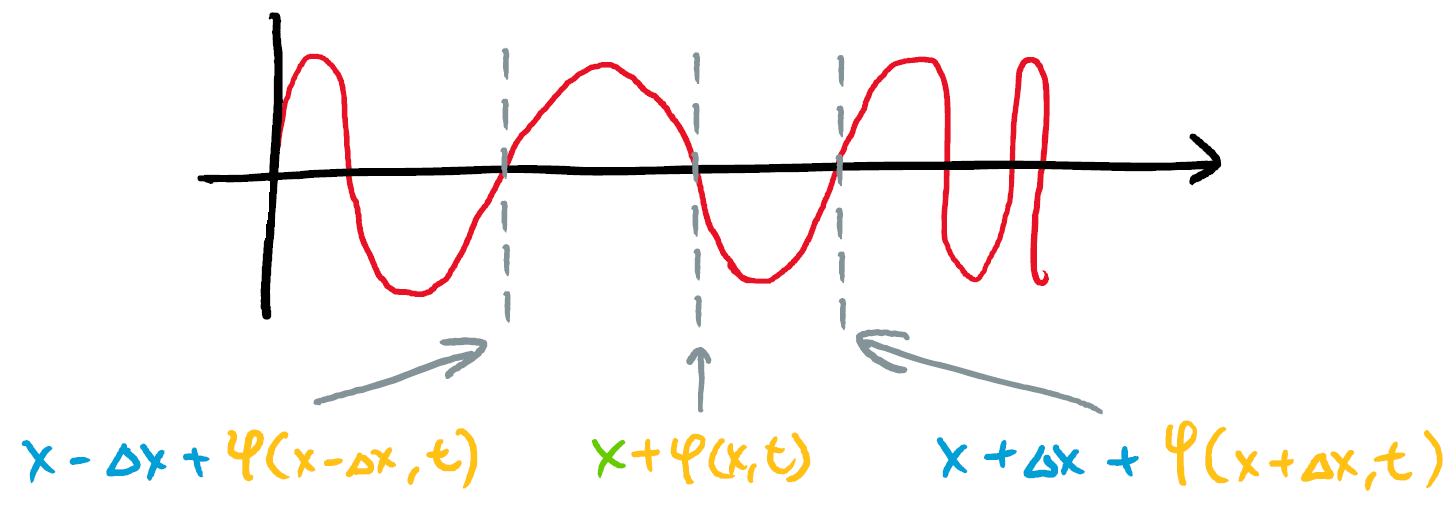
\includegraphics[width=\textwidth]{long2}
        \end{minipage}
    \end{center}

\end{itemize}

Longitudinal wave is \red{displacement of slinky segments} at different position / time,
described by the function $\Psi(x,t)$.\\

\bf{\ul{Deriving wave eqauation}}

\begin{enumerate}

    \item Although a slinky is a continuous line of mass, 
    we can divide it into many very small segments and only model the motions of the center of these segments - 
    using their centers as nodes to represent the motion of the segment.

    \begin{itemize}
        \item The mass of a segment concentrate at its center. 
        We only need to consider the velocity and acceleration on the nodes.

        \begin{center}
            \begin{minipage}{0.8\linewidth}
                \centering
                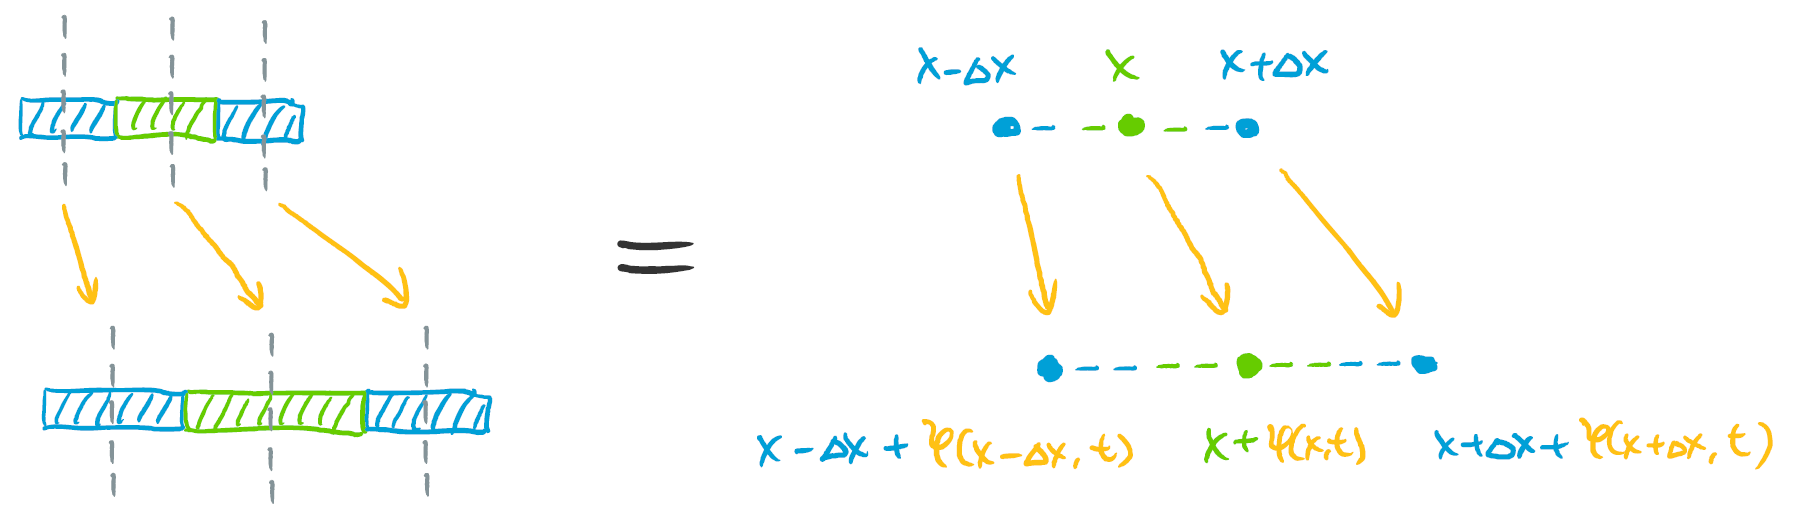
\includegraphics[width=\textwidth]{long_node}
            \end{minipage}
        \end{center}

        \item Interaction between segments are like elastic forces $\sim kx$ between nodes. 
        You can think of it as a spring-mass system composed of infinitely many masses.

        \begin{center}
            \begin{minipage}{0.7\linewidth}
                \centering
                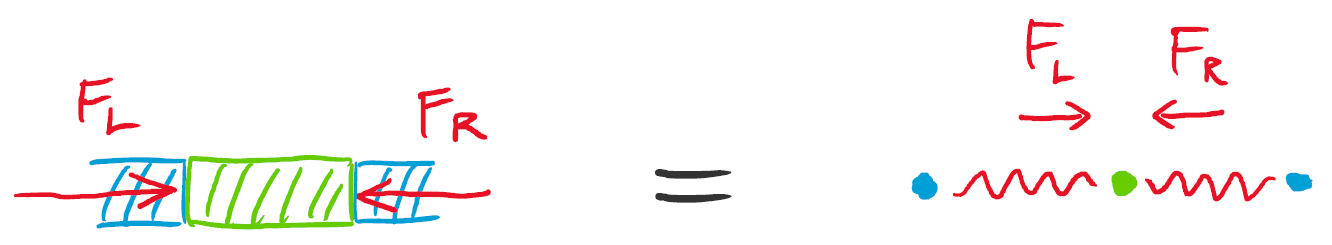
\includegraphics[width=\textwidth]{long_force}
            \end{minipage}
        \end{center}

    \end{itemize}


    \item Consider 3 neighbouring nodes.
    When a longitudinal wave is travelling through, 
    their displacements are described by the function $\Psi(x,t)$. 
    We can compute the change of separation between nodes.

    \hfill\\[-3em]
    \begin{center}
        \begin{tikzpicture}
            \matrix(m)[matrix of nodes,
                nodes={align=center},
                %row 1/.style={anchor=south},
                %column 1/.style={nodes={text width=2cm,align=right}}
            ]{
                Node's position & Left node & Center node & Right node \\
                $\mstack{\text{When static}}$ & $x-\Delta x$ & $x$ & $x+\Delta x$ \\
                $\mstack{\text{When a wave is}\\\text{travelling through}}$ & $x-\Delta x +\yellow{\Psi(x-\Delta x,t)}$ 
                    & $x+\yellow{\Psi(x,t)}$ & $x+\Delta x + \yellow{\Psi(x+\Delta x,t)}$\\
            };
            \draw (m-1-1.south west) to (m-1-4.south east);
            \draw (m-1-1.north east -| m-3-1.south east) to (m-3-1.south east);
            \draw (m-1-2.north east -| m-3-2.south east) to (m-3-2.south east);
            \draw (m-1-3.north east -| m-3-4.south west) to (m-3-4.south west);
            %
            \draw[draw=blue] ($(m-3-2.south) + (-8ex,0)$) to ($(m-3-2.south) + (-6ex,-2ex)$) 
                to node[pos=0.5,blue,below]{\begin{tabular}{c} Their distance in-between\\[-1.5ex] increases by\\[-1.5ex] $\Psi(x,t)-\Psi(x-\Delta x, t)$ \end{tabular}} 
                ($(m-3-3.south) + (-4ex,-2ex)$) to ($(m-3-3.south) + (-2ex,0)$);
            \draw[draw=blue] ($(m-3-4.south) + (8ex,0)$) to ($(m-3-4.south) + (6ex,-2ex)$) 
                to node[pos=0.5,blue,below]{\begin{tabular}{c} Their distance in-between\\[-1.5ex] increases by\\[-1.5ex] $\Psi(x+\Delta x,t)-\Psi(x, t)$ \end{tabular}} 
                ($(m-3-3.south) + (4ex,-2ex)$) to ($(m-3-3.south) + (2ex,0)$);
        \end{tikzpicture}
    \end{center}

    \item The elastic force on the center node is proportional to the separation change with its neighbouring nodes,
    just like the elastic force in spring, $F=-k(\Delta L)$.  
    But here we express the elastic force using \bf{Young's modulus}:
    \aleq{
        (\text{Elastic force}) = F = -Y\cdot \qty(\frac{\Delta L}{L}) = -Y\cdot \qty(\frac{\text{Change in length}}{\text{Original length}})
    }

    So the elastic forces on the two sides of the center node are:
    \aleq{
        \bcase{
            F_L &= -Y\cdot \frac{\Psi(x,t)-\Psi(x-\Delta x, t)}{\Delta x}\\[1ex]
            %
            F_R &= -Y\cdot \frac{\Psi(x+\Delta x,t)-\Psi(x, t)}{\Delta x}
        }
    }
    
\end{enumerate}
\begin{notation}[Side note:]

    Spring constant $k$ depends on the length of the material. 
    For example, we can compute the equivalent spring constants for two springs in series to be half of the original.
    \begin{center}
        \begin{minipage}{0.5\linewidth}
            \centering
            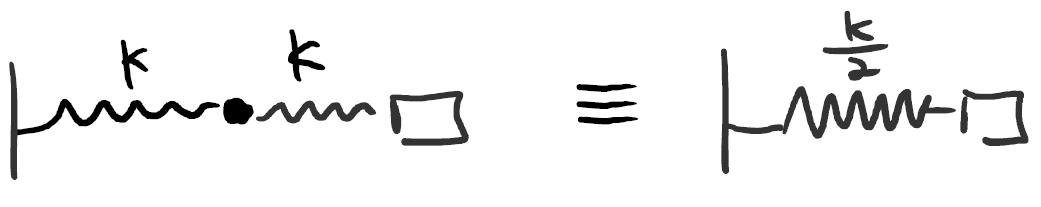
\includegraphics[width=\textwidth]{spring}
        \end{minipage}
    \end{center}
    If we stack more springs in series, we can see that $k\propto \qty(\inv{\text{Length of material}})$. 
    To remove this dependency on length, we define the Young's modulus, 
    which is a property that only depends on the material's type. 
    \aleq{
        \Aboxed{
            F = -k(\Delta L) = -\frac{Y}{L}(\Delta L) 
        }
    }

\end{notation}

\newpage
\begin{enumerate}
    \item[4.] The Newton's \nth{2} Law on the center segment's center is therefore
    \begin{center}
        \begin{minipage}{0.25\linewidth}
            \centering
            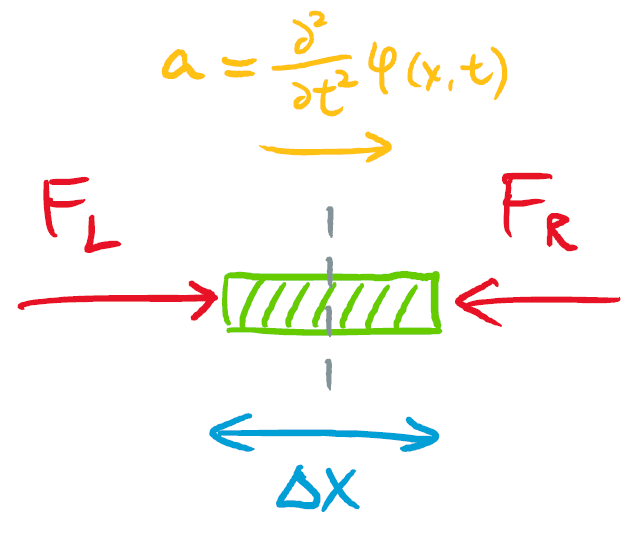
\includegraphics[width=\textwidth]{long_freebody}
        \end{minipage}
    \end{center}

    \addArrow[red]{dt2psi}{(2ex,4ex)}
    {\scriptsize Horizontal acceleration\\[-1ex]\scriptsize = \nth{2} derivative of \\[-1ex]\scriptsize segment's displacement over $t$}
    {(2ex,3ex)}{(-15ex,0)}
    \addArrow[yellow]{mu2}{(-2ex,-4ex)}
    {\scriptsize $\mu = $ Density per unit length\\[-1ex]\scriptsize $\Rightarrow \mu\Delta x = $ Mass of the segment}
    {(0,-1ex)}{(-3ex,-1ex)}
    \addArrow[green]{dxpsi1}{(3ex,5.5ex)}{\scriptsize \nth{1} derivative of $x$}{(0,3ex)}{(8ex,-3ex)}
    \addArrow[green]{dxpsi2}{(12ex,5.5ex)}{}{(0,3ex)}
    \addBentArrow*[blue]{dx2psi}{(13ex,6ex)}
    {\scriptsize This is just the derivative $\frac{f(x+\Delta x)-f(x)}{\Delta x}$\\[-1ex]\scriptsize $\Rightarrow$ become \nth{2} derivative over $x$}
    {(6ex,0.5ex)}{(12ex,-5ex)}
    \aleq{
        m\cul[red]{a_\rightarrow} &= F_L - F_R \\[1em]
        %
        (\tkn{mu2}{\cul[yellow]{\mu}}\Delta x)\tkn{dt2psi}{\cul[red]{\pdvv[2]{t}\Psi(x,t)}} 
            &= Y \qty[\cul[green]{\frac{\Psi(x+\Delta x,t)-\Psi(x, t)}{\Delta x}} 
                - \cul[green]{\frac{\Psi(x,t)-\Psi(x-\Delta x, t)}{\Delta x}}]\\[1em]
        %
        &= Y \qty[\tkn{dxpsi1}{\cul[green]{\pdv{x}\Psi(x,t)\eval_{\text{at }x+\Delta x}}} 
            - \tkn{dxpsi2}{\cul[green]{\pdv{x}\Psi(x,t)\eval_{\text{at }x}}}] \\[1.5em]
        %
        \mu \pdvv[2]{t}\Psi(x,t)
        &= Y \  \cub[blue]{\dfrac{\eval{\pdvv{x}\Psi(x,t)}_{\cbox[blue]{\scriptstyle\text{at }x+\Delta x}} 
            - \eval{\pdvv{x}\Psi(x,t)}_{\cbox[blue]{\scriptstyle\text{at }x}}}{\cbox[blue]{\Delta x}}}{} \\
        %
        &= Y \tkn{dx2psi}{\cul[blue]{\pdvv[2]{x}\Psi(x,t)}}\\[1em]
        %
        \Aboxed{
            \frac{\mu}{Y}\pdvv[2]{t}\Psi(x,t) &= \pdvv[2]{x}\Psi(x,t)
        }
    }
    
    
\end{enumerate}

Compare with the general form of wave equation $\dinv{v^2}\pdvv[2]{t}y(x,t) = \pdvv[2]{x}y(x,t)$,
we can identify the wave speed of longitudinal wave as 
\aleq{
    v=\sqrt{\frac{\mu}{Y}} = \sqrt{\frac{\text{Mass per Length}}{\text{Young's modulus}}}
}




\linesep
\newpage
% Section %%%%%%%%%%%%%%%%%%%%%%%%%%%%%%%%%%%%%%%%%%%%%%%%%%%%
\section{Wave Equation \& Initial Value Problem}

The initial value problem is asking the follow: 
If we are told the state of a system at the start, 
how will system evolve at later time?\\

For example in wave propagation, 
given that at $t=0$, 
a string is hold to a shape described by the function $\Psi(x,0)$. 
After released, how will the waveform evolve? 

\begin{center}
    \begin{minipage}{0.25\linewidth}
        \centering
        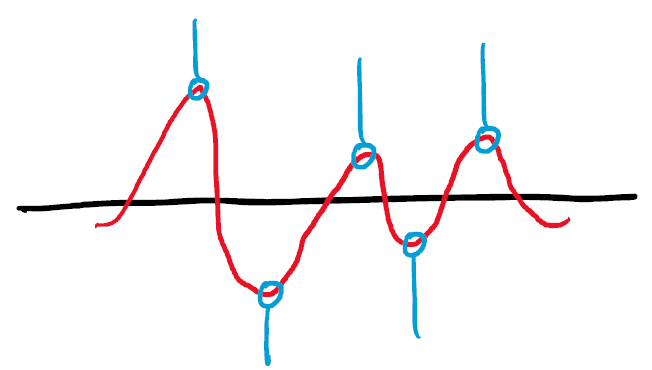
\includegraphics[width=\textwidth]{init1}
    \end{minipage}
    $\qquad\Rightarrow\qquad$
    \begin{minipage}{0.25\linewidth}
        \centering
        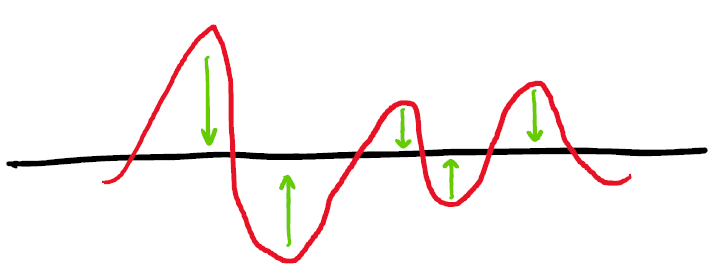
\includegraphics[width=\textwidth]{init2}
    \end{minipage}
    $\qquad\Rightarrow\qquad$
    \begin{minipage}{0.1\linewidth}
        \centering
        \red{\huge ?}
    \end{minipage}
\end{center}

We would like to solve $\cub[blue]{\Psi(x,t)}{\substack{\text{the waveform}\\\text{in the future}}}$ 
by the given $\cub[blue]{\Psi(x,0)}{\substack{\text{the waveform}\\\text{at the start}}}$ 
and $\cub[blue]{\pdvv{t}\Psi(x,t)\eval_{t=0}}{\substack{\text{velocity at each point}\\\text{at the start}}}$.


%%%%%%%%%%%%%%
\subsection{General Solution to Wave Equation}

The wave equation is a \bf{partial differential equation} (PDE):
\aleq{
    \pdvv[2]{x}\Psi(x,t) = \dinv{v^2}\pdvv[2]{t}\Psi(x,t)
}

We can show that the general solution is
\aleq{
    \Aboxed{
        \Psi(x,t) = f(x+vt) + g(x-vt)
    }
}

where $f(\cdots)$ and $g(\cdots)$ are any single variable function,
and then we substitute $x+vt$ or $x-vt$ as the inputs.
For example,
\aleq{
    f(u) = \sin u + u^2 \quad\Rightarrow\quad f(x+vt) = \sin(x+vt) + (x+vt)^2
}

\begin{proof}
    By differentiation with chain rule. 
    \begin{center}
        \begin{minipage}{0.45\textwidth}
            \centering
            \ul{L.H.S.}
            \aleq{
                \pdvv{x} f(x+vt) 
                &=  \pdvv{f(u)}{u}\eval_{u=x+vt}\pdvv{(x+vt)}{x} \\[1ex]
                &= \pdvv{f(u)}{u}\eval_{u=x+vt} \cdot 1 \\[1em]
                %
                \pdvv[2]{x} f(x+vt) 
                &=  \pdvv[2]{f(u)}{u}\eval_{u=x+vt}\pdvv{(x+vt)}{x} \\[1ex]
                &= \pdvv[2]{f(u)}{u}\eval_{u=x+vt} \cdot 1
            }
        \end{minipage}
        \hfill
        \vline
        \hfill
        \begin{minipage}{0.45\textwidth}
            \centering
            \ul{R.H.S.}
            \aleq{
                \dinv{v^2}\pdvv{t} f(x+vt) 
                &= \dinv{v^2}\pdvv{f(u)}{u}\eval_{u=x+vt}\pdvv{(x+vt)}{t} \\[1ex]
                &= \dinv{v^2}\pdvv{f(u)}{u}\eval_{u=x+vt} \cdot v \\[1em]
                %
                \dinv{v^2}\pdvv[2]{t} f(x+vt) 
                &=  \dinv{v}\pdvv[2]{f(u)}{u}\eval_{u=x+vt}\pdvv{(x+vt)}{t} \\[1ex] 
                &= \dinv{v}\pdvv[2]{f(u)}{u}\eval_{u=x+vt} \cdot v
            }
        \end{minipage}
    \end{center}
    \hfill\\
    Obviously L.H.S = R.H.S.. You can also prove the same for $g(x-vt)$.
\end{proof}


\bf{\ul{Physical Interpretation}}

\begin{itemize}
    \item $f(x+vt)$ : When $t$ increases, need to decrease $x$ to maintain the same value of $f$.\\
    \phantom{$f(x+vt)$ : }$\Rightarrow$ This is a waveform travelling in the $-x$ direction with speed $v$.

    \item $g(x-vt)$ : When $t$ increases, need to increase $x$ to maintain the same value of $f$.\\
    \phantom{$g(x-vt)$ : }$\Rightarrow$ This is a waveform travelling in the $+x$ direction with speed $v$.
\end{itemize}

When they come to each other, they join together (superposition) to create a new waveform. 

\begin{center}
    \begin{minipage}{0.35\linewidth}
        \centering
        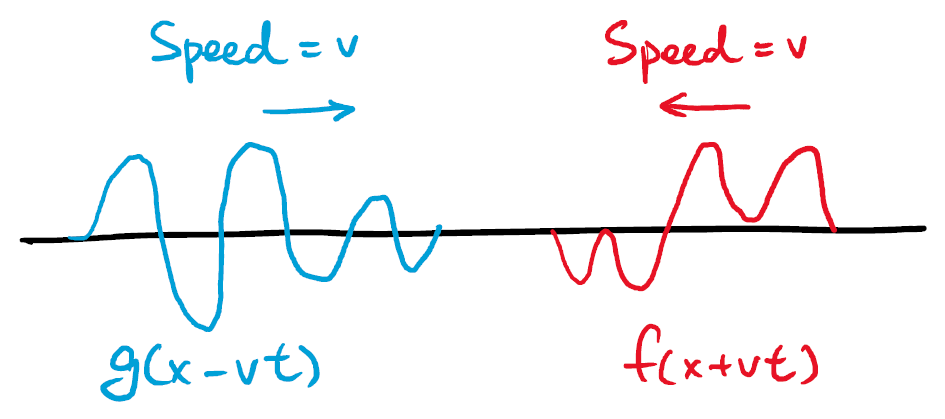
\includegraphics[width=\textwidth]{super1}
    \end{minipage}
    $\qquad\xRightarrow{\substack{\text{Waves collide}\\\text{=}\\\text{Superposition}}}\qquad$
    \begin{minipage}{0.35\linewidth}
        \centering
        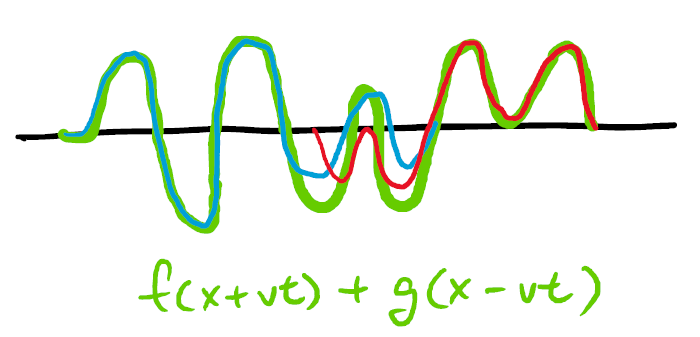
\includegraphics[width=\textwidth,trim=0 0 0 -3em]{super2}
    \end{minipage}
\end{center}


\vskip 1em
%%%%%%%%%%%%%%
\subsection{Solution to Initial Value Problem}

\it{(This derivation is long but not important. Welcome to skip to the result.)}

\begin{enumerate}
    \item From the initial conditions, break them down by $\Psi=f+g$.
    \aleqr{
        \Psi(x,0) &= f(x+0) + g(x-0) \label{eq:fg0}\\[1em]
        \pdvv{t}\Psi(x,t)\eval_{t=0} &= v\dvv{f(u)}{u}\eval_{u=x+0} - v\dvv{g(u)}{u}\eval_{u=x-0} \label{eq:dfg0}
    }

    \vskip 1ex
    \item Differentiate Eq.\eqref{eq:fg0} with respect to $x$:
    \aleqr{
        \dvv{x}\Psi(x,0) = \dvv{f(u)}{u}\eval_{u=x+0} + \dvv{g(u)}{u}\eval_{u=x-0} \label{eq:fg1}
    }

    \vskip 1ex
    \item Isolate $\dvv{f(u)}{u}\eval_{u=x+0}$ and $\dvv{g(u)}{u}\eval_{u=x-0}$ 
    from Eq.\eqref{eq:fg1} and Eq.\eqref{eq:dfg0}.
    \aleqr{
        \text{Eq.\eqref{eq:fg1}} +\dinv{v} (\text{Eq.\eqref{eq:dfg0}})
        &\qquad\Rightarrow\qquad
        \dvv{f(u)}{u}\eval_{u=x+0} = \half\qty[\dvv{x}\Psi(x,0) + \dinv{v}\pdvv{t}\Psi(x,t)\eval_{t=0}]
        \label{eq:df0}
        \\[1em]
        %
        \text{Eq.\eqref{eq:fg1}} -\dinv{v} (\text{Eq.\eqref{eq:dfg0}})
        &\qquad\Rightarrow\qquad
        \dvv{g(u)}{u}\eval_{u=x-0} = \half\qty[\dvv{x}\Psi(x,0) - \dinv{v}\pdvv{t}\Psi(x,t)\eval_{t=0}]
        \label{eq:dg0}
    }

    \newpage
    \item Integrate both Eq.\eqref{eq:df0} and Eq.\eqref{eq:dg0}.
    \addArrow[red]{C1}{(0,6ex)}{\scriptsize $C_1 = $ some integration constant}
    {(2ex,3ex)}{(12ex,-3.5ex)}
    \addArrow[red]{C2}{(0,6ex)}{\scriptsize $C_2 = $ some integration constant}
    {(2ex,3ex)}{(12ex,-3.5ex)}
    \aleq{
        \text{Eq.\eqref{eq:df0}} 
        \qquad\Rightarrow\qquad 
        \int \dvv{f(u)}{u}\eval_{u=x+0} \dd{x} 
        &= \half\int\qty[\cul[red]{\dvv{x}\Psi(x,0)} + \dinv{v}\pdvv{t}\Psi(x,t)\eval_{t=0}]\dd{x} \\[1.2em]
        %
        \int \dvv{f(x)}{x} \dd{x} 
        &= \half\qty[\tkn{C1}{\cul[red]{\Psi(x,0) + C_1}} + \dinv{v}\int\qty[\pdvv{t}\Psi(x,t)\eval_{t=0}]\dd{x}] \\[0.8em]
        %
        f(x) &= \half \biggl[\Psi(x,0) + C_1 
            + \dinv{v}\cub[green]{\int_{\green{s=0}}^{\green{s=x}}\qty[\pdvv{t}\Psi(\green{s},t)\eval_{t=0}]\dd{\green{s}}}
            {\substack{s \text{ = A dummy variable to replace }x\\\text{For convenience in later steps}}}\biggr]\\[1em]
        %
        \text{Eq.\eqref{eq:dg0}} 
        \qquad\Rightarrow\qquad 
        \int \dvv{g(u)}{u}\eval_{u=x-0} \dd{x} 
        &= \half\int\qty[\cul[red]{\dvv{x}\Psi(x,0)} - \dinv{v}\pdvv{t}\Psi(x,t)\eval_{t=0}]\dd{x} \\[1.2em]
        %
        \int \dvv{g(x)}{x} \dd{x} 
        &= \half\qty[\tkn{C2}{\cul[red]{\Psi(x,0) + C_2}} - \dinv{v}\int\qty[\pdvv{t}\Psi(x,t)\eval_{t=0}]\dd{x}] \\[0.8em]
        %
        g(x) &= \half \biggl[\Psi(x,0) + C_2 
            - \dinv{v}\cub[green]{\int_{\green{s=0}}^{\green{s=x}}\qty[\pdvv{t}\Psi(\green{s},t)\eval_{t=0}]\dd{\green{s}}}
            {\substack{s \text{ = A dummy variable to replace }x\\\text{For convenience in later steps}}}\biggr]
    }

    \vskip 1ex
    \item Replace the "$x$" in $f(x)$ by "$x+vt$", and the "$x$" in $g(x)$ by "$x-vt$".
    \aleq{
        f(\blue{x+vt}) &= \half \qty[\Psi(\blue{x+vt},0) + C_1 
            + \dinv{v}\int_{s=0}^{s=\blue{x+vt}}\qty[\pdvv{t}\Psi(s,t)\eval_{t=0}]\dd{s}]\\[0.5em]
        %
        g(\blue{x-vt}) &= \half \qty[\Psi(\blue{x-vt},0) + C_1 
            - \dinv{v}\int_{s=0}^{s=\blue{x-vt}}\qty[\pdvv{t}\Psi(s,t)\eval_{t=0}]\dd{s}]
    }

    \vskip 1ex
    \item Add these two expression together to give $\Psi(x,t)$
    \addArrow[yellow]{combine_bound}{(-8ex,8ex)}{\scriptsize Combine integral by their bounds}
    {(-3ex,2ex)}{(18ex,-4.5ex)}
    \addArrow[yellow]{combine_bound}{(-56ex,9ex)}{}{(-3.5ex,1ex)}{(19ex,-2.5ex)}
    \aleq{
        \Psi(x,t) &= f(x+vt) + g(x-vt) \\
        %
        &= \half\qty[\Psi(x+vt,0) + \Psi(x-vt,0)] + \half (C_1+C_2) \\
        &\qquad + \dinv{2v} \int_{s=0}^{s=x+vt} \qty[\pdvv{t}\Psi(s,t)\eval_{t=0}]\dd{s} 
            \cub[yellow]{- \dinv{2v} \int_{s=0}^{s=x-vt}}{\substack{\text{Can switch}\\\text{upper/lower bound}\\\text{and change sign}}} 
                \qty[\pdvv{t}\Psi(s,t)\eval_{t=0}]\dd{s}\\
        %
        &= \half\qty[\Psi(x+vt,0) + \Psi(x-vt,0)] + \half (C_1+C_2) \\
        &\qquad + \dinv{2v} \int_{s=0}^{s=x+vt} \qty[\pdvv{t}\Psi(s,t)\eval_{t=0}]\dd{s} 
            \yellow{+} \dinv{2v} \int_{\yellow{s=x-vt}}^{\yellow{s=0}} \qty[\pdvv{t}\Psi(s,t)\eval_{t=0}]\dd{s}\\[1.5em]
        %
        &= \half\qty[\Psi(x+vt,0) + \Psi(x-vt,0)] + \half (C_1+C_2) + \dinv{2v}\tkn{combine_bound}{\cul[yellow]{\int_{s=x-vt}^{s=x+vt}}} \qty[\pdvv{t}\Psi(s,t)\eval_{t=0}]\dd{s} 
    }
    

    \item Finally, substitute $t=0$ to find out what $C_1+C_2$ is.
    \aleq{
        \Psi(x,\red{0}) &= \half\qty[\Psi(x+\red{0},\red{0}) + \Psi(x-\red{0},\red{0})] 
            + \half (C_1+C_2) + \dinv{2v}\int_{s=x-\red{0}}^{s=x+\red{0}} \qty[\pdvv{t}\Psi(s,t)\eval_{t=0}]\dd{s} \\[1em]
        %
        &= \half\qty[\Psi(x,\red{0}) + \Psi(x,\red{0})] + \half (C_1+C_2) + 0 \\[1em]
        %
        C_1+C_2 &= 0
    }

\end{enumerate}

Finally, we reach the solution to the initial value problem of wave equation.
\aleq{
    \Aboxed{
        \cub[blue]{\Psi(x,t)}{\substack{\text{the waveform}\\\text{in the future}}} 
        = \half\cub[red]{\qty[\Psi(x+vt,0) + \Psi(x-vt,0)]}
            {\substack{\text{Derived from the}\\\text{initial waveform }\Psi(x,0)}} 
            + \dinv{2v}\cub[green]{\int_{s=x-vt}^{s=x+vt} \qty[\pdvv{t}\Psi(s,t)\eval_{t=0}]\dd{s}}
            {\substack{\text{Derived from the}\\\text{initial velocity }\pdv{t}\Psi(s,t)\eval_{t=0}}}
    }
}


\begin{example}
    Given the initial waveform of the string as
    \aleq{
        \Psi(x,0) = \begin{cases}
            b-\dfrac{b\abs{x}}{a} & \text{for }\abs{x}\leq a \\[1ex]
            0 & \text{for }\abs{x}>a
        \end{cases}
    }
    and knowing that the string is static at the beginning (i.e. velocity $= 0$ everywhere).

    \begin{center}
        \begin{minipage}{0.3\linewidth}
            \centering
            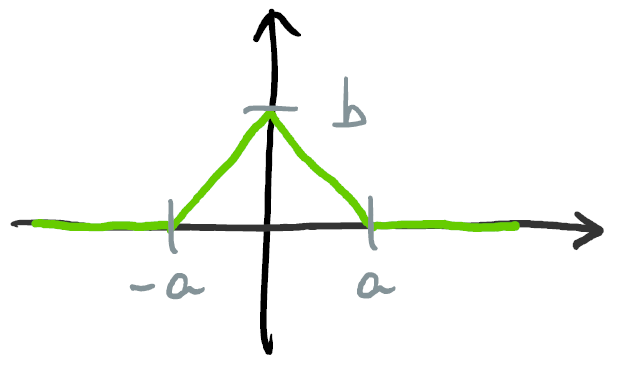
\includegraphics[width=\textwidth]{init_eg}
        \end{minipage}
    \end{center}

    We can find how the wave will evolve by direct substituting these info into the general solution.
    \aleq{
        \Psi(x,t) &= \half\qty[\Psi(x+vt) + \Psi(x-vt)] 
            + \dinv{2v}\int_{x-vt}^{x+vt} \cut[yellow]{\ccancelto[yellow]{0}{\qty[\pdvv{t}\Psi(s,t)\eval_{t=0}]}}{\text{Because no initial velocity}}\dd{s}\\[1ex]
        %
        &= \cub[red]{\half\qty(b-\frac{b\abs{x+vt}}{a})}{\substack{\text{This is a function of }x+vt\\\text{i.e. the waveform travelling}\\\text{in }-\text{ve direction}}} 
        + \cub[blue]{\half\qty(b-\frac{b\abs{x-vt}}{a})}{\substack{\text{This is a function of }x-vt\\\text{i.e. the waveform travelling}\\\text{in }+\text{ve direction}}} 
        + 0
    }

    \begin{center}
        \begin{minipage}{0.3\linewidth}
            \centering
            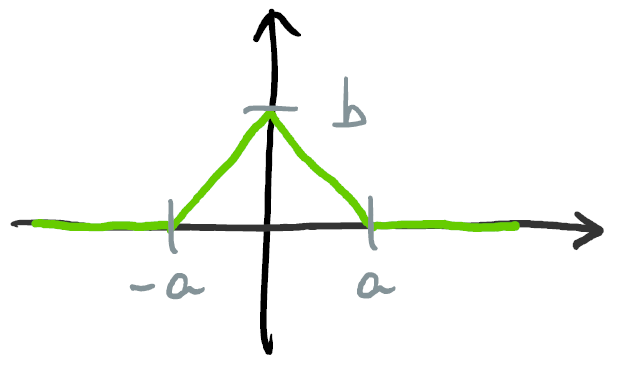
\includegraphics[width=\textwidth]{init_eg}
        \end{minipage}
        $\qquad\xRightarrow{\text{After release}}\qquad$
        \begin{minipage}{0.3\linewidth}
            \centering
            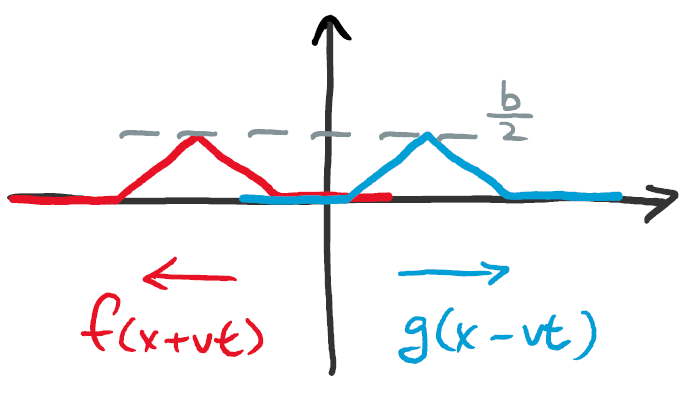
\includegraphics[width=\textwidth, trim=0 0 0 -4em]{init_eg2}
        \end{minipage}
    \end{center}

\end{example}


\linesep
% Section %%%%%%%%%%%%%%%%%%%%%%%%%%%%%%%%%%%%%%%%%%%%%%%%%%%%
\section{Boundary Value Problem \& Standing Wave}

The boundary value problem is asking the follow: 
If we are only given the value of the function at the end points and the initial state, 
how will system evolve at later time?

\begin{center}
    E.g. 
    \hspace{0.05\textwidth}
    \begin{minipage}{0.25\linewidth}
        \centering
        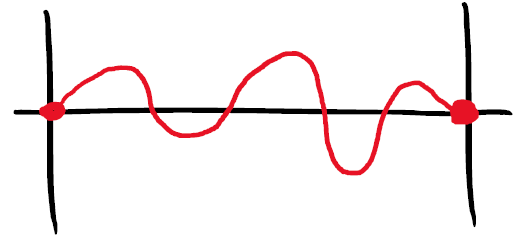
\includegraphics[width=\textwidth]{stand1}
    \end{minipage}
    \hspace{0.05\textwidth}
    \begin{minipage}{0.25\linewidth}
        \centering
        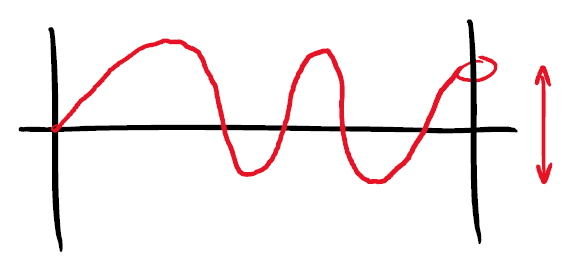
\includegraphics[width=\textwidth]{stand2}
    \end{minipage}
\end{center}

In a standing wave configuraton, 
a string is usually tied at both ends (or free ends). 
It is very important to know: \cul[red]{what kinds of "vibration pattern" are allowed?}

\begin{center}
    \begin{minipage}{0.25\linewidth}
        \centering
        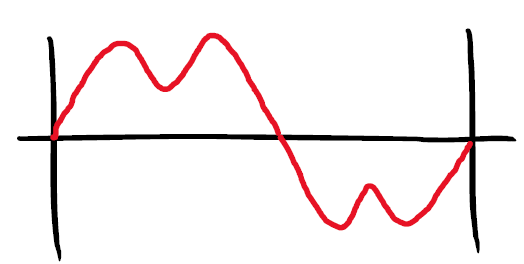
\includegraphics[width=\textwidth]{stand_weird1}
    \end{minipage}
    $\quad\Rightarrow\quad$
    \begin{minipage}{0.25\linewidth}
        \centering
        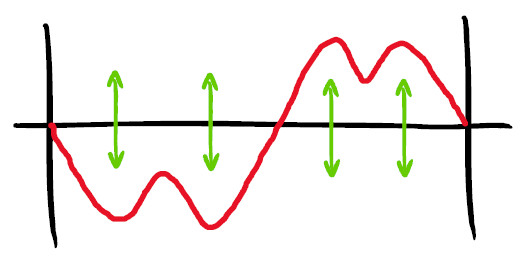
\includegraphics[width=\textwidth]{stand_weird2}
    \end{minipage}
    {\LARGE \ or\ } 
    \begin{minipage}{0.25\linewidth}
        \centering
        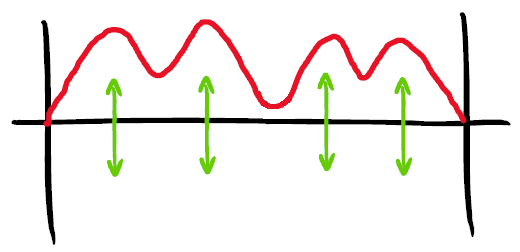
\includegraphics[width=\textwidth]{stand_weird3}
    \end{minipage}
    {\LARGE \ ?\ } 
\end{center}

And if the standing wave starts in a shape described by the function $\Psi(x,0)$. 
After releasing, how will the waveform evolves? 




%%%%%%%%%%%%%%
\subsection{The Method of Separation of Variables}

Here introduces an alternative method to solve the wave equation 
- \bf{method of separation of variables}. 
We first assume the solution to be able to be written as a product of 2 single variable function,
one as a function position $x$ and the other as a function of time $t$.
\aleq{
    \Psi(x,t) = \tkn{Xx}{\blue{X(x)}}\tkn{Tt}{\red{T(t)}}
}
\addArrow[blue]{Xx}{(-3ex,-3ex)}
{\scriptsize This part only\\[-1ex]\scriptsize depends on $x$}
{(-1ex,-1ex)}{(0,-1ex)}
\addArrow[red]{Tt}{(3ex,-3ex)}
{\scriptsize This part only\\[-1ex]\scriptsize depends on $t$}
{(1ex,-1ex)}{(0,-1ex)}

\vskip 1em
Substitute into the equation,
\aleq{
    \pdvv[2]{x}[\blue{X(x)}\red{T(t)}] &= \inv{v^2}\pdvv[2]{t}[\blue{X(x)}\red{T(t)}]\\[1ex]
    %
    \tkn{Tt2}{\red{T(t)}}\pdvv[2]{x}[\blue{X(x)}] &= \inv{v^2}\tkn{Xx2}{\blue{X(x)}}\pdvv[2]{t}[\red{T(t)}]
}
\addArrow[blue]{Xx2}{(0,-3ex)}
{\scriptsize $X(x)$ not depends on $t$.\\[-0.5ex]\scriptsize Can be taken out of $\pdv[2]{t}$}
{(0,-1ex)}{(0,-1.2ex)}
\addArrow[red]{Tt2}{(0,-3ex)}
{\scriptsize $T(t)$ not depends on $x$.\\[-0.5ex]\scriptsize Can be taken out of $\pdv[2]{x}$}
{(0,-1ex)}{(0,-1.2ex)}

\vskip 2em
Rearrange so that the L.H.S is a function of $x$ only, 
and R.H.S. is a function of $t$ only.
\aleq{
    \cub[blue]{\dinv{\blue{X(x)}}\pdvv[2]{x}[\blue{X(x)}]}{\text{only contain }x} 
    &= \cub[red]{\inv{v^2}\dinv{\red{T(t)}}\pdvv[2]{t}[\red{T(t)}]}{\text{only contain t}} 
    = \tkn{k2}{\qty(\mstack{\text{Some}\\\text{Constant}})} = \green{-k^2}
}
\addArrow[green]{k2}{(0,-8ex)}
{The only possibility for two functions\\of different variables to be identical\\is when both equal to a constant}
{(0,-2ex)}{(0,-2ex)}


The constant is written as $-k^2$ is just for convenience.
We can now split the part with $x$ and the part with $t$,
forming two independent \nth{2} order linear ODEs. 
\aleq{
    \bcase{
        \dinv{\blue{X(x)}}\pdvv[2]{x}[\blue{X(x)}] &= \green{-k^2}
        \qquad\Rightarrow\qquad 
        \pdvv[2]{x}\blue{X(x)} + \green{k^2}\blue{X(x)} = 0\\
        %
        \inv{v^2}\dinv{\red{T(t)}}\pdvv[2]{t}[\red{T(t)}] &= \green{-k^2}
        \qquad\Rightarrow\qquad 
        \pdvv[2]{t}\red{T(t)} + v^2\green{k^2}\red{T(t)} = 0\\
    }
}

You should be very farmiliar with this kind of ODE - 
the equation of motion of SHM. Their solutions are 
\aleq{
    \bcase{
        \blue{X(x)} &= C\cos{(kx)} + D\sin{(kx)} \\
        \red{T(t)} &= A\cos{(kvt)} + B\sin{(kvt)}
    }
}

where $A,B,C,D$ are constants to be determined 
from the boundary conditions and initial conditions.


%%%%%%%%%%%%%%
\subsection{Boundary Conditions \& Solutions}

In standing wave, 
the boundary condition at the ends of the string can be either fixed 
or free to move up / down. 
Here introduces two most common boundary conditions,
and their corresponding solutions.

%%%%%%%%%%%%%%
\subsubsection{Dirichlet Condition}

\begin{center}
    \begin{minipage}{0.25\linewidth}
        \centering
        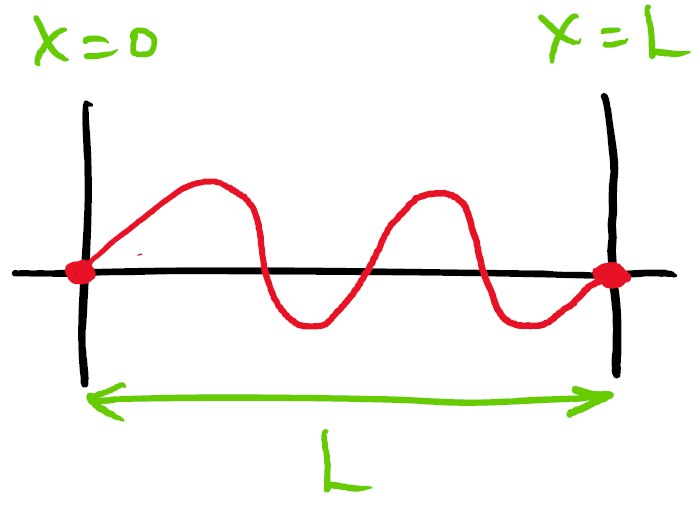
\includegraphics[width=\textwidth]{dirichlet}
    \end{minipage}
\end{center}

The \bf{Dirichlet condition} in standing wave is having \bf{2 fixed ends},
i.e. requires the magnitude at both ends to be fixed at $0$ (at any time $t$).
If the string is of length $L$, it writes:
\aleq{
    \Aboxed{
        \bcase{
            \Psi(0,t) &= 0\\
            \Psi(L,t) &= 0
        }
    }
} 


By these conditions, we must have $X(0)=X(L)=0$.
\begin{itemize}
    \item At $x=0$, $X(0)=C\cos(0)+D\sin(0) = 0$. 
    It holds only if $C=0$.
    
    \item At $x=L$, $X(L)= D\sin(kL) = 0$. 
    It holds only if $kL=n\pi$, with $n=\tkn{dirichlet0}{\gray{0}},1,2,3,...$.\\
    \addArrow[gray]{dirichlet0}{(3ex,3ex)}
    {\scriptsize $n=0$ is technically an answer,\\[-1ex] \scriptsize but it gives $X(x)=D\sin 0 = 0$,\\[-1ex]\scriptsize meaning the string cannot shake at all.}
    {(1ex,2ex)}{(7ex,2.5ex)}
\end{itemize}

So we require $k=\dfrac{n\pi}{L}$. 
Substitute it into $X(x)$ and $T(t)$, 
\aleq{
    \bcase{
        \blue{X(x)} &= D\sin{\qty(\dfrac{n\pi}{L}x)} \\
        \red{T(t)} &= A\cos{\qty(\dfrac{n\pi}{L}vt)} + B\sin{\qty(\dfrac{n\pi}{L}vt)}
    }
}

For each integer $n=1,2,3...$, we can construct one set of $\Psi(x,t)$:
\aleq{
    \Psi_\green{n}(x,t) &= \blue{X_\green{n}(x)}\red{T_\green{n}(t)} \\
    &= \blue{\biggl[}\sin\qty(\frac{\green{n}\pi}{L}x)\blue{\biggr]}
        \red{\biggl[}A_\green{n}\cos\qty(\frac{\green{n}\pi}{L}vt) 
            + B_\green{n}\sin\qty(\frac{\green{n}\pi}{L}vt)\red{\biggr]}
}

Then by the superposition property of linear equations, 
the general solution is the (linear) combination of all possible solutions.
\aleq{
    \Aboxed{
        \Psi(x,t) = \sum_{\green{n=1}}^{\green{\infty}}
            \blue{\biggl[}\sin\qty(\frac{\green{n}\pi}{L}x)\blue{\biggr]}
            \red{\biggl[}A_\green{n}\cos\qty(\frac{\green{n}\pi}{L}vt) 
                + B_\green{n}\sin\qty(\frac{\green{n}\pi}{L}vt)\red{\biggr]}
        %
        \qquad (\text{Dirichlet Condition})
    }
}

All the constants $A_n$, $B_n$ shall be determined only after an initial condition is given.

%%%%%%%%%%%%%%
\subsubsection{Neumann Condition}

\begin{center}
    \begin{minipage}{0.25\linewidth}
        \centering
        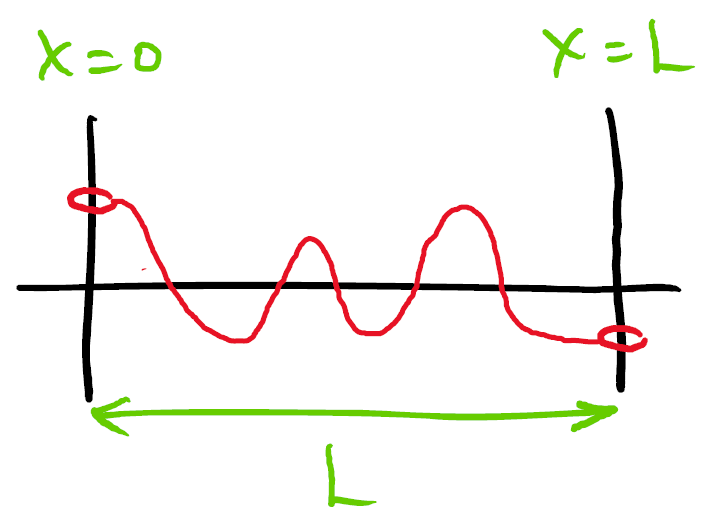
\includegraphics[width=\textwidth]{neumann}
    \end{minipage}
\end{center}

The \bf{Neumann condition} in standing wave is having \bf{2 free ends} - 
the end segments are free to move up and down.
To achieve so, the ends' holdings must not exert any vertical force at the end segment 
(otherwise the ends are not freely moving with the string body.) 

\begin{center}
    \hspace{0.1\textwidth}
    \begin{minipage}{0.18\linewidth}
        \centering
        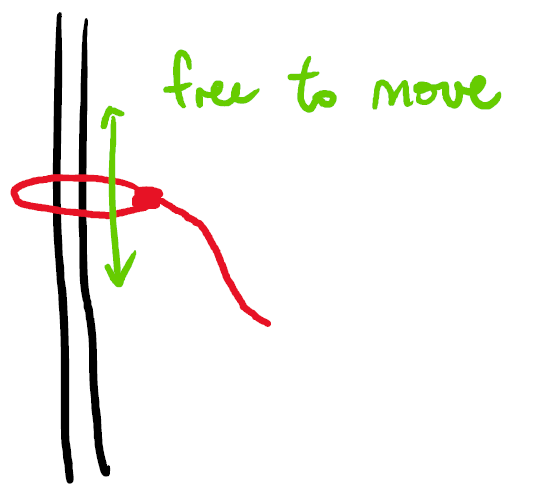
\includegraphics[width=\textwidth]{neumann_end2}
    \end{minipage}
    $\qquad\Rightarrow\qquad$
    \begin{minipage}{0.35\linewidth}
        \centering
        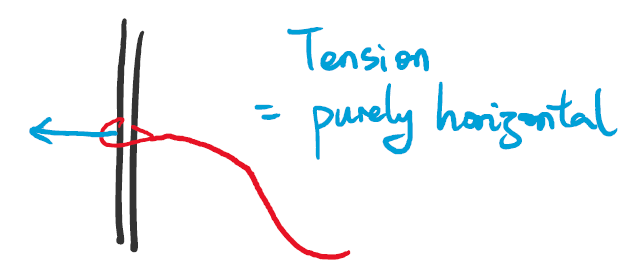
\includegraphics[width=\textwidth]{neumann_end1}
    \end{minipage}
\end{center}

Having only horizontal force on the end segments means that the slopes at both ends are be $0$ (at any time $t$).
If the string is of length $L$, it writes:
\aleq{
    \Aboxed{
        \bcase{
            \pdvv{x}\Psi(x,t)\eval_{x=0} &= 0\\
            \pdvv{x}\Psi(x,t)\eval_{x=L} &= 0
        }
    }
} 



By these conditions, we must have $\eval{\dvv{X(x)}{x}}_{x=0}=\eval{\dvv{X(x)}{x}}_{x=L}=0$.

\begin{itemize}
    \item At $x=0$, $\eval{\dvv{X(x)}{x}}_{x=0}=-C\sin(0)+D\cos(0) = 0$. 
    It holds only if $D=0$.
    
    \item At $x=L$, $\eval{\dvv{X(x)}{x}}_{x=L}= -C\sin(kL) = 0$. 
    It holds only if $kL=n\pi$, with $n=\tkn{neumann0}{0},1,2,3,...$.\\
    \addArrow[gray]{neumann0}{(0,-3ex)}
    {\scriptsize This time we can keep $n=0$,\\[-1ex] \scriptsize because it gives $X(x)=C\cos 0 = C$.\\[-1ex]\scriptsize Motion is retained in $T(t)$.}
    {(0,-1ex)}{(-3ex,-2.5ex)}

\end{itemize}

So we require $k=\dfrac{n\pi}{L}$. 
Notice that 
\begin{itemize}
    \item when $k\neq 0$, we can substitute it into $X(x)$ and $T(t)$, 
    \aleq{
        \bcase{
            \blue{X(x)} &= C\cos{\qty(\dfrac{n\pi}{L}x)} \\
            \red{T(t)} &= A\cos{\qty(\dfrac{n\pi}{L}vt)} + B\sin{\qty(\dfrac{n\pi}{L}vt)}
        }
    }

    \item but when $k=0$, the solution of $X(t)$ and $T(t)$ become
    \aleq{
        \blue{X(x)}= C
        \qquad\text{and}\qquad
        \barray{r@{\extracolsep{0.5ex}}l}{
            \pdvv[2]{t}\red{T(t)}&= 0\\
            \Rightarrow\quad \red{T(t)}&= At + B
        }
    }
\end{itemize}

For each integer $n=0,1,2,3...$, we can construct one set of $\Psi(x,t)$:
\aleq{
    \Psi_\green{n}(x,t) &= \blue{X_\green{n}(x)}\red{T_\green{n}(t)} \\
    &= \begin{cases}
        \blue{\biggl[}1\blue{\biggr]}
            \red{\biggl[}A_\green{0}t + B_\green{0}\red{\biggr]}
        & \text{for }\green{n}=0 \\[1em]
        %
        \blue{\biggl[}\cos\qty(\frac{\green{n}\pi}{L}x)\blue{\biggr]} 
            \red{\biggl[}A_\green{n}\cos\qty(\frac{\green{n}\pi}{L}vt) + B_\green{n}\sin\qty(\frac{\green{n}\pi}{L}vt)\red{\biggr]}
        &\text{for }\green{n}>0
    \end{cases}
}

Then by the superposition property of linear equations, 
the general solution is the (linear) combination of all possible solutions.
\aleq{
    \Aboxed{
        \Psi(x,t) = \red{\biggl[}A_\green{0}t + B_\green{0}\red{\biggr]}
        + \sum_{\green{n=1}}^{\green{\infty}} 
            \blue{\biggl[}\cos\qty(\frac{\green{n}\pi}{L}x)\blue{\biggr]}
            \red{\biggl[}A_\green{n}\cos\qty(\frac{\green{n}\pi}{L}vt) 
                + B_\green{n}\sin\qty(\frac{\green{n}\pi}{L}vt)\red{\biggr]}
        %
        \quad (\text{Neumann Condition})
    }
}

All the constants $A_n$, $B_n$ shall be determined only after an initial condition is given.

\vskip 1em
\begin{exercise}
    We can carry out similar steps to obtain the general solution in other combination of boundary conditions.
    \begin{enumerate}
        \item Use $x=0$ 's condition to elimiate one of $C$ or $D$.
        \item Use $x=L$ 's condition to determine what values of $k$ can be.
        \item Substitute $k$'s value into $\Psi(x,t)=\blue{X(x)}\red{T(t)}$.
        \item The general solution is the linear combination of $\Psi(x,t)$ of all possible $k$.
    \end{enumerate}

    As a practice, you may try to derive for the case with one fixed end and one open end.

    \begin{center}
        \begin{minipage}{0.25\linewidth}
            \centering
            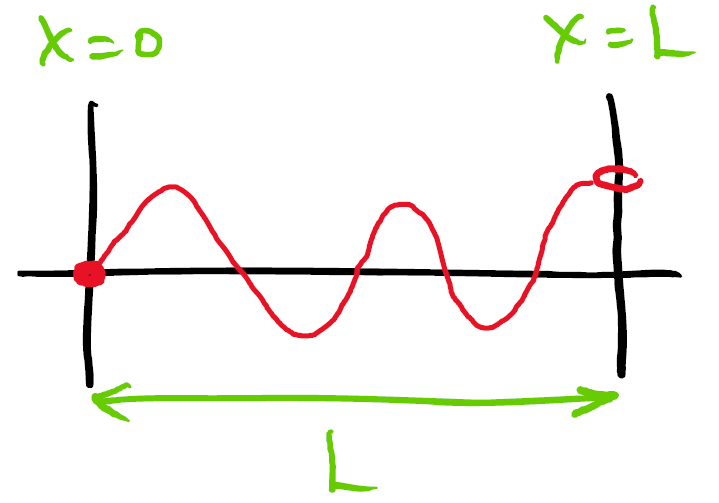
\includegraphics[width=\textwidth]{fix_free}
        \end{minipage}
    \end{center}

    You should get 
    \aleq{
        \Aboxed{
            \Psi(x,t) = \sum_{\green{n=1}}^{\green{\infty}}
                \blue{\biggl[}\sin\qty(\green{\frac{2n-1}{2}}\frac{\pi}{L}x)\blue{\biggr]}
                \red{\biggl[}A_\green{n}\cos\qty(\green{\frac{2n-1}{2}}\frac{\pi}{L}vt) 
                    + B_\green{n}\sin\qty(\green{\frac{2n-1}{2}}\frac{\pi}{L}vt)\red{\biggr]}
        }
    }

\end{exercise}


%%%%%%%%%%%%%%
\subsection{Modes of Standing Wave}

Observing that the general solution is a superposition of all simplier solutions of different $n$.
Each $n$ has its corresponding $X_n(x)$ and $T_n(t)$.
\aleq{
    \Psi(x,t) = \sum_{\green{n}}\Psi_\green{n}(x,t) 
        = \sum_{\green{n}}\qty[\blue{X_\green{n}(x)}\red{T_\green{n}(t)}]
}

\begin{itemize}
    \item $\blue{X_\green{n}(x)}$ is only about variation by position $x$ 
        - Carry info about the \blue{waveform}.
    \item $\red{T_\green{n}(t)}$ is only about variation by time $t$ 
        - Carry info about the \red{time evolution}.
\end{itemize}

Each $\Psi_\green{n}(x,t)$ is \bf{a unique set of vibration pattern} in standing wave,
and they evolve independently from each other.
Therefore we call them the \bf{normal modes} of standing wave.
\aleq{
    \text{i.e.}\qquad \qty(\mstack{\text{The n\Nth mode}\\\Psi_\green{n}(x,t)})
    = \blue{\qty(\mstack{\text{Waveform of}\\\text{the n\Nth mode}\\X_\green{n}(x)})} \times 
        \red{\qty(\mstack{\text{Time evolution}\\\text{of the n\Nth mode}\\T_\green{n}(t)})}
}

\vskip 1ex
We can draw the graphs for each $\Psi_n(x,t)$. {\scriptsize (Here frequency = angular frequency $\omega$)}
\begin{center}
    \begin{tabular}{>{\centering\arraybackslash}m{4ex}|
            >{\centering\arraybackslash}m{0.28\linewidth}|
            >{\centering\arraybackslash}m{0.28\linewidth}|
            >{\centering\arraybackslash}m{0.28\linewidth}}
        & Dirichlet (2 fixed ends) & Neumann (2 free ends) & 1 fixed-1 free end\\
        \hline
        n=0 &
        \begin{tabular}[c]{@{}c@{}}
            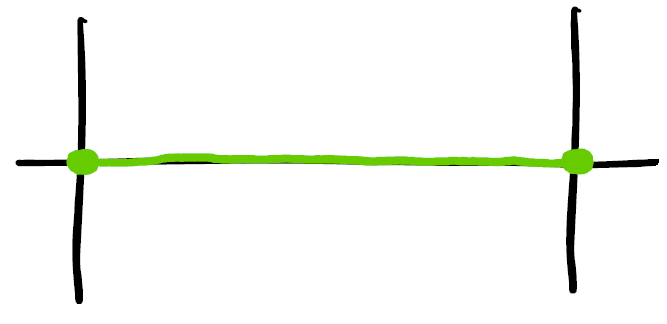
\includegraphics[width=\linewidth]{mode_D0}\\[-1.5ex]
            \blue{$X(x)=0$}\\[-1.5ex]
            So $\Psi(x,t)=0$.\\[-1.5ex]
            Nothing moves.
        \end{tabular}
        &
        \begin{tabular}[c]{@{}c@{}}
            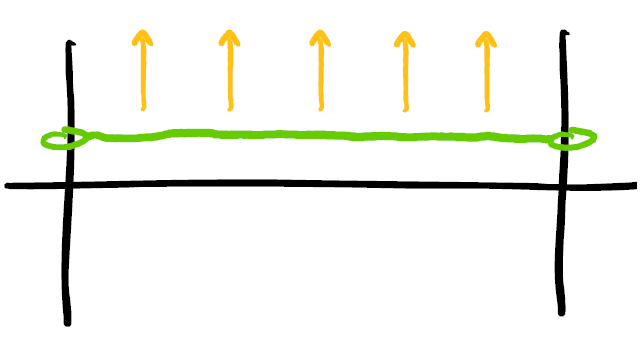
\includegraphics[width=\linewidth]{mode_N0}\\[-1.5ex]
            \blue{$X(x)=$ const. = flat line}\\[-1.5ex]
            \red{$T(t)= At + B$} \\[-1.5ex]
            $\Psi(x,t)=$ whole line moves\\[-1.5ex]
            up/down at constant speed
        \end{tabular}
        &
        \begin{tabular}[c]{@{}c@{}}
            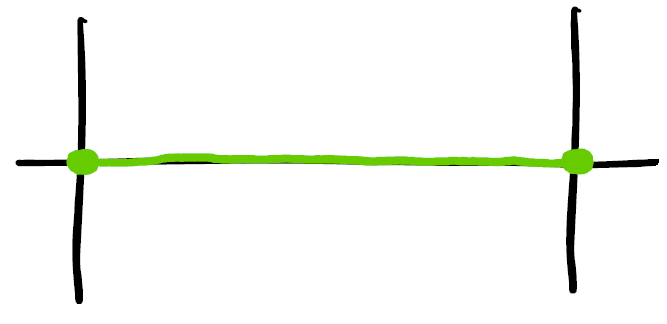
\includegraphics[width=\linewidth]{mode_D0}\\[-1.5ex]
            \blue{$X(x)=0$}\\[-1.5ex]
            So $\Psi(x,t)=0$.\\[-1.5ex]
            Nothing moves.
        \end{tabular}
        \\
        %
        \hline
        n=1 &
        \begin{tabular}[c]{@{}c@{}}
            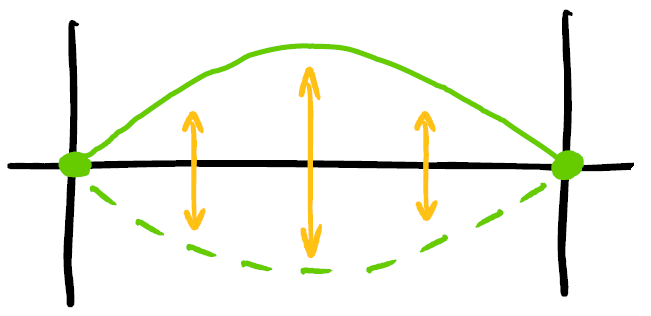
\includegraphics[width=\linewidth]{mode_D1}\\[-1.5ex]
            \blue{$X(x)$ : Shape = 0.5 sine}\\[-0.8ex]
            \red{$T(t)$ : Frequency = $\dfrac{\pi v}{L}$}\\[1ex]
        \end{tabular}
        &
        \begin{tabular}[c]{@{}c@{}}
            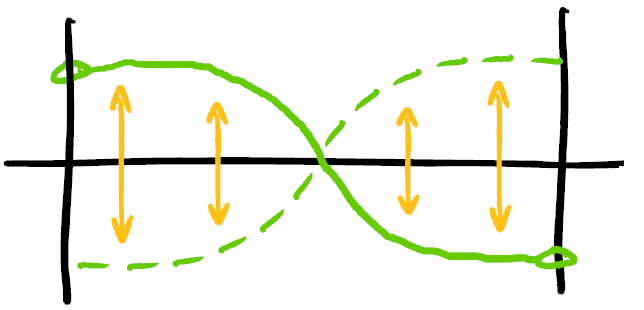
\includegraphics[width=\linewidth]{mode_N1}\\[-1.5ex]
            \blue{$X(x)$ : Shape = 0.5 cosine}\\[-0.8ex]
            \red{$T(t)$ : Frequency = $\dfrac{\pi v}{L}$}\\[1ex]
        \end{tabular}
        &
        \begin{tabular}[c]{@{}c@{}}
            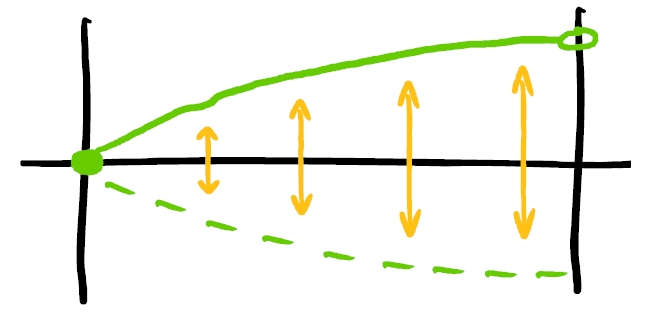
\includegraphics[width=\linewidth]{mode_O1}\\[-1.5ex]
            \blue{$X(x)$ : Shape = 0.25 sine}\\[-0.8ex]
            \red{$T(t)$ : Frequency = $\dfrac{\pi v}{2L}$}\\[1ex]
        \end{tabular}
        \\
        %
        \hline
        n=2 &
        \begin{tabular}[c]{@{}c@{}}
            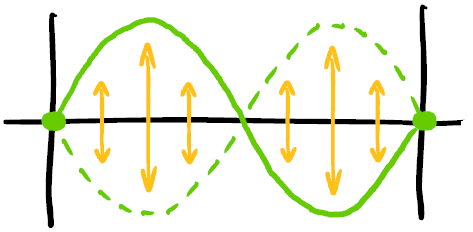
\includegraphics[width=\linewidth]{mode_D2}\\[-1.5ex]
            \blue{$X(x)$ : Shape = full sine}\\[-0.5ex]
            \red{$T(t)$ : Frequency = $\dfrac{2\pi v}{L}$}\\[1ex]
        \end{tabular}
        &
        \begin{tabular}[c]{@{}c@{}}
            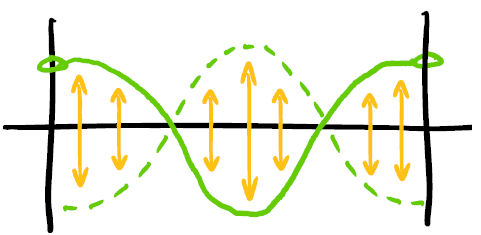
\includegraphics[width=\linewidth]{mode_N2}\\[-1.5ex]
            \blue{$X(x)$ : Shape = full cosine}\\[-0.5ex]
            \red{$T(t)$ : Frequency = $\dfrac{2\pi v}{L}$}\\[1ex]
        \end{tabular}
        &
        \begin{tabular}[c]{@{}c@{}}
            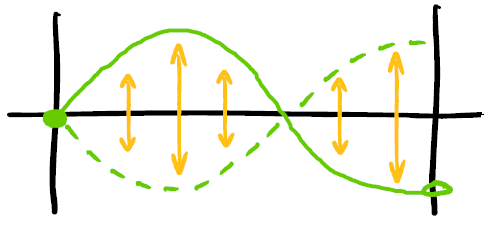
\includegraphics[width=\linewidth]{mode_O2}\\[-1.5ex]
            \blue{$X(x)$ : Shape = 0.75 sine}\\[-0.5ex]
            \red{$T(t)$ : Frequency = $\dfrac{3\pi v}{2L}$}\\[1ex]
        \end{tabular}
    \end{tabular}
    \\
    $\vdots$\\
     and so on.
\end{center}

Here I shall emphasize: 
\cul[red]{\bf{The combination of standing wave's pattern (waveform) and}} \cul[red]{\bf{vibration frequency (time evolution) is fixed}}
- It is impossible to let the string vibrate in one of the above patterns but at a different frequency.\\

When we encounter a wave pattern that is not in one of the normal wave's waveform,
we must first break it down into a sum of different normal modes.
For example

\begin{center}
    \begin{minipage}{0.5\linewidth}
        \centering
        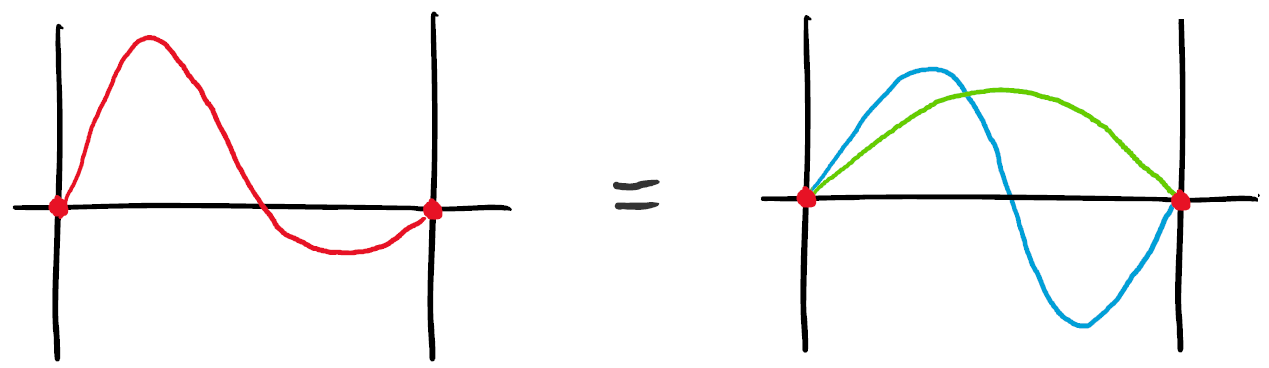
\includegraphics[width=\textwidth]{sum}
    \end{minipage}
    \ = \ (\green{\nth{1} mode}) + (\blue{\nth{2} mode})
\end{center}

Because each mode has its own vibration frequency, 
the resulted wave will not maintain a regular shape like the initial waveform.
\begin{center}
    \begin{tabular}{>{\centering\arraybackslash}m{13ex}|
        >{\centering\arraybackslash}m{0.2\linewidth}|
        >{\centering\arraybackslash}m{0.2\linewidth}|
        >{\centering\arraybackslash}m{0.2\linewidth}|
        >{\centering\arraybackslash}m{0.15\linewidth}}
        & $t=0$ & $t=\dfrac{L}{2v}$ & $t=\dfrac{L}{v}$ \\[1ex]
        \hline
        \makecell{\green{\nth{1} mode}\\ Period $= \dfrac{2L}{v}$}
        &
        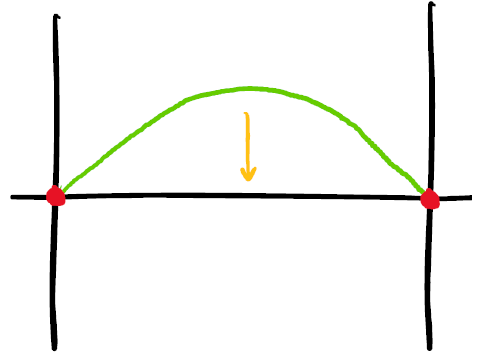
\includegraphics[width=\linewidth]{sum_11}
        &
        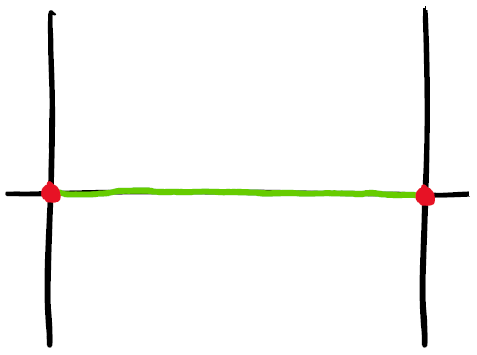
\includegraphics[width=\linewidth]{sum_12}
        &
        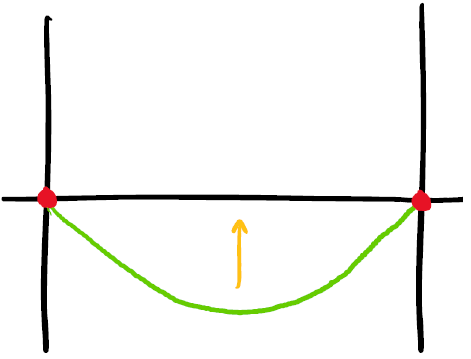
\includegraphics[width=\linewidth]{sum_13}
        &
        \green{Only completed $\frac{1}{2}$ of its period}
        \\[1ex]
        %
        \hline
        \makecell{\blue{\nth{2} mode}\\ Period $= \dfrac{L}{v}$}
        &
        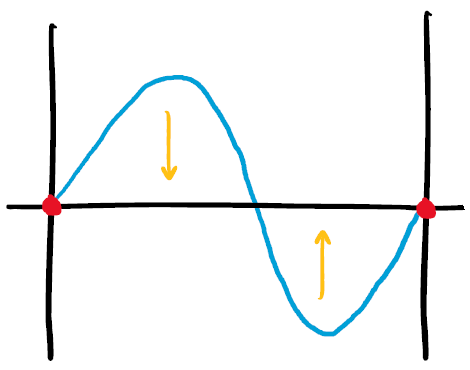
\includegraphics[width=\linewidth]{sum_21}
        &
        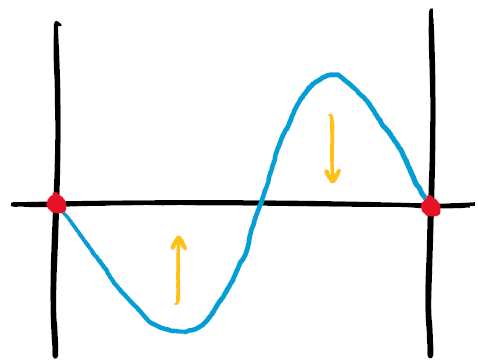
\includegraphics[width=\linewidth]{sum_22}
        &
        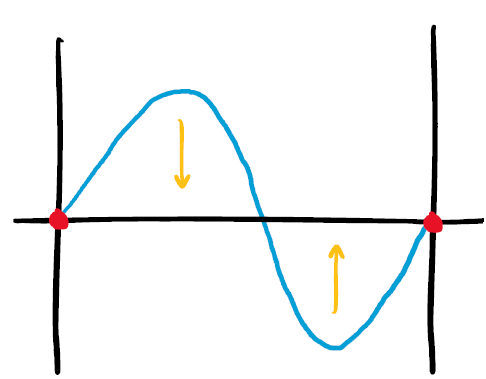
\includegraphics[width=\linewidth]{sum_23}
        &
        \blue{Already completed 1 full period}
        \\[1ex]
        %
        \hline
        \red{Sum}
        & 
        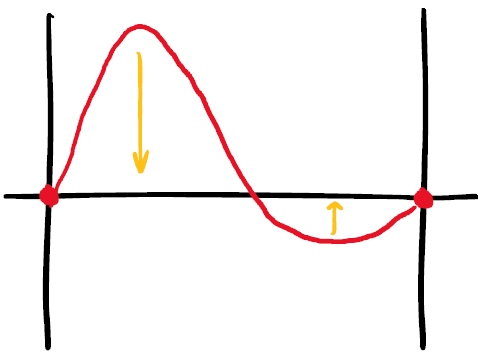
\includegraphics[width=\linewidth]{sum_31}
        &
        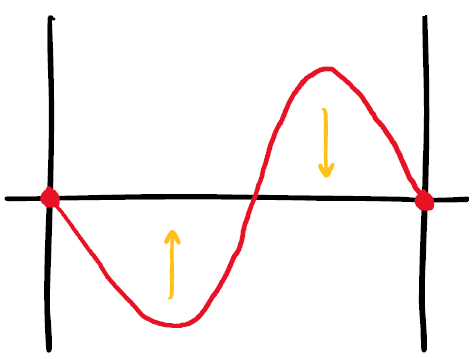
\includegraphics[width=\linewidth]{sum_32}
        &
        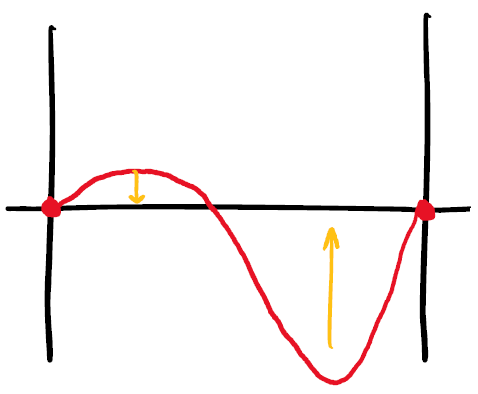
\includegraphics[width=\linewidth]{sum_33}
        &
        \makecell{\red{Irregular pattern}\\[1ex] Period \\ = follow the\\ lowest mode}
    \end{tabular}
\end{center}



%%%%%%%%%%%%%%
\subsection{Fourier Series}

So if we are given some arbituary pattern as the initial wave form,
how can we break it down into normal modes mathematically? 
The tool is called \bf{Fourier Series}.\\

Denote a periodic function as $f(x) = f(x+L)$, 
which has a period $L$,

\begin{center}
    \begin{minipage}{0.4\linewidth}
        \centering
        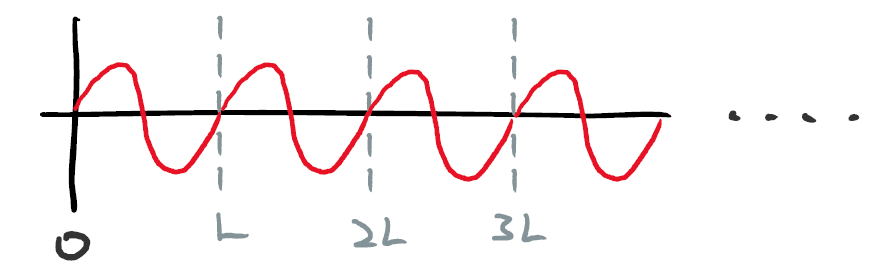
\includegraphics[width=\textwidth]{periodic}
    \end{minipage}
\end{center}

it can be expanded as a series of sin and cosine terms:
\aleq{
    \Aboxed{
        f(x) = \frac{{a_0}}{2} 
            + \sum_{n=1}^{\infty} \qty[{a_n}\cos\qty(\frac{2\pi n}{L}x)
            + {b_n}\sin\qty(\frac{2\pi n}{L}x)]
    }
}

The \bf{Fourier coefficients} $a_n$ (including $a_0$) and $b_n$ can be calculated by these integrals:
\begin{empheq}[box=\fbox]{align*}
    a_n &= \frac{2}{L} \int^L_0 f(x) \cdot \cos\qty(\frac{2\pi n}{L}x) \dd{x} \\[1ex]
    b_n &= \frac{2}{L} \int^L_0 f(x) \cdot \sin\qty(\frac{2\pi n}{L}x) \dd{x}
\end{empheq}

\begin{proof}
    The above formulas work thanks to these integral properties.
    For any integer $m,n$,
    \aleq{
        \int^{2\pi}_0 \cos(mx)\cos(nx) \dd{x} &= 
        \begin{cases}
            2\pi & \text{if }m=n=0\\
            \pi & \text{if }m=n\neq 0\\
            0 & \text{if }m\neq n    
        \end{cases}\\
        %
        \int^{2\pi}_0 \sin(mx)\sin(nx) \dd{x} &= 
        \begin{cases}
            0 & \text{if }m=n=0\\
            \pi & \text{if }m=n\neq 0\\
            0 & \text{if }m\neq n    
        \end{cases}\\
        %
        \int^{2\pi}_0 \sin(mx)\cos(nx) \dd{x} &= 0
    }

    i.e. the integral $=0$ whenever $m\neq n$ or the $\sin$ / $\cos$ does not match.
    Let's have a demonstration using $\cos\qty(\dfrac{2\pi n}{L}x)$ with $n\geq 1$.
    \aleq{
        &\int^L_0 f(x)\cos\qty(\dfrac{2\pi \blue{n}}{L}x) \dd{x}\\
        %
        = &\int^L_0 \qty[\frac{a_\red{0}}{2} 
            + \sum_{m=1}^{\infty} \qty[a_\red{m}\cos\qty(\frac{2\pi \red{m}}{L}x)
            + b_\red{m}\sin\qty(\frac{2\pi \red{m}}{L}x)]] \cos\qty(\dfrac{2\pi \blue{n}}{L}x) \dd{x}\\
        %
        = &\int^L_0 \biggl[
            \cub[green]{\frac{a_\red{0}}{2} \cos\qty(\dfrac{2\pi \blue{n}}{L}x)}
                {\substack{\text{Integrate }\cos\\\text{for 1 period}\\=0}} 
            + \sum_{m=1}^{\infty} a_\red{m}\cub[red]{\cos\qty(\frac{2\pi \red{m}}{L}x)\cos\qty(\dfrac{2\pi \blue{n}}{L}x)}
                {\substack{\cos \text{ and }\cos\\ \text{Integral }\neq 0 \text{ only if }m=n}}
            + \sum_{m=1}^{\infty} b_\red{m}\cub[blue]{\sin\qty(\frac{2\pi \red{m}}{L}x)\cos\qty(\dfrac{2\pi \blue{n}}{L}x)}
                {\substack{\sin \text{ and }\cos\\ \text{Integral always gives }0}}\biggr]\dd{x}\\
        %
        = &\int^L_0 a_\blue{n}\cos\qty(\dfrac{2\pi \blue{n}}{L}x)\cos\qty(\dfrac{2\pi \blue{n}}{L}x) \dd{x} \\
        %
        = &\,a_\blue{n}\cdot \frac{L}{2}
    }
    \hfill\\[-4em]
    \aleq{
        \Rightarrow \qquad a_\blue{n} = \dfrac{2}{L}\int^L_0 f(x)\cos\qty(\dfrac{2\pi \blue{n}}{L}x) \dd{x} 
    }
    As an exercise, you can also prove the same formula for $b_n$.

\end{proof}


\begin{example}
    Evolution of square wave \\

    Given the function of a periodic square wave as 
    \aleq{
        f(x) = \begin{cases}
        1 &\text{for }0<x<\frac{L}{2} \\
        -1 &\text{for }\frac{L}{2}<x<L
        \end{cases}
    }

    \begin{center}
        \begin{minipage}{0.6\linewidth}
            \centering
            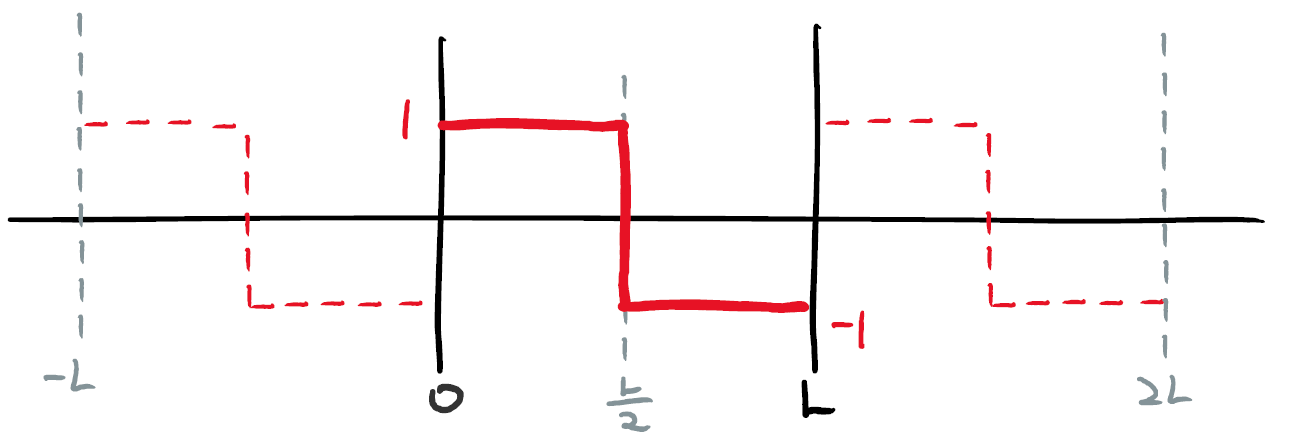
\includegraphics[width=\textwidth]{square}
        \end{minipage}
    \end{center}

    The Fourier coefficients can be directly computed:
    \aleq{
        a_n &= \frac{2}{L}\int_0^{\frac{L}{2}} \red{1}\cdot \cos\qty(\frac{2\pi n}{L}x) \dd{x}
            + \frac{2}{L}\int_{\frac{L}{2}}^L \red{-1}\cdot \cos\qty(\frac{2\pi n}{L}x) \dd{x}\\[1ex]
        %    
        &= 0 \\[1ex]
        %
        b_n &= \frac{2}{L}\int_0^{\frac{L}{2}} \red{1}\cdot \sin\qty(\frac{2\pi n}{L}x) \dd{x}
            + \frac{2}{L}\int_{\frac{L}{2}}^L \red{-1}\cdot \sin\qty(\frac{2\pi n}{L}x) \dd{x}\\[1ex]
        %
        &= \frac{2}{n\pi}[1-(-1)^n] = 
        \begin{cases}
            0 &\text{for }n=\text{even}\\
            \dfrac{4}{n\pi} &\text{for }n=\text{odd}    
        \end{cases}
    }

    So its Fourier series write as
    \aleq{
        f(x) = \frac{4}{\pi}\qty[\cul[green]{
            \cul[yellow]{
                \tkn{sq1}{\cul[blue]{\sin(\frac{2\pi}{L}\cdot x)}} 
                + \dinv{3}\tkm{sq2}\sin(\frac{2\pi}{L}\cdot 3x)} 
            + \tkm{sq3}\dinv{5}\sin(\frac{2\pi}{L}\cdot 5x)} + \dots]
    }
    \addArrow[blue]{sq1}{(0,-3ex)}{First mode}{(0,-3ex)}
    \addArrow[yellow]{sq2}{(0,-5.5ex)}{First 2 modes}{(0,-3.2ex)}
    \addArrow[green]{sq3}{(0,-8ex)}{First 3 modes}{(0,-3.5ex)}{(0,1ex)}

    \vskip 3em
    \begin{center}
        \begin{minipage}{0.8\linewidth}
            \centering
            \includegraphics[width=\textwidth]{square_mode}
        \end{minipage}
    \end{center}

    At this point, we have already obtained each $\blue{X_\green{n}(x)}$ as
    \aleq{
        \blue{X_\green{n}(x)} =  \dfrac{4}{n\pi}\sin\qty(\frac{2\pi n}{L}x)
        \qquad {\scriptstyle(\text{odd }n\text{ only})}
    }

    To complete the n\Nth normal mode, 
    multiply $\red{T_\green{n}(t)}$ of the corresponding $n$.
    \aleq{
        \Psi_\green{n}(x,t) = \blue{X_\green{n}(x)}\red{T_\green{n}(t)} 
        = \blue{\biggl[}\dfrac{4}{\green{n}\pi}\sin\qty(\frac{2\pi \green{n}}{L}x)\blue{\biggr]}
        \red{\biggl[}A_\green{n} \cos \qty(\frac{2\pi \green{n}}{L}vt) 
            + B_\green{n}\sin \qty(\frac{2\pi \green{n}}{L}vt) \red{\biggr]}
    }
    
    Finally, the general evolution is the sum of all normal modes.
    \begin{empheq}[box=\fbox]{align*}
        \Psi(x,t) = \sum_{n=1}^{\infty}\Psi_\green{n}(x,t) 
        &= \sum_{n=1}^{\infty}\blue{X_\green{n}(x)}\red{T_\green{n}(t)} \\
        &= \sum_{\text{odd }n\text{ only}}^{\infty}\blue{\biggl[}\dfrac{4}{\green{n}\pi}\sin\qty(\frac{2\pi \green{n}}{L}x)\blue{\biggr]}
        \red{\biggl[}A_\green{n} \cos \qty(\frac{2\pi \green{n}}{L}vt) 
            + B_\green{n}\sin \qty(\frac{2\pi \green{n}}{L}vt) \red{\biggr]}
    \end{empheq}

    To exactly determine the constants $A_n,B_n$,
    an initial condition is required. 
    For example, \ul{if we specify that the string is static before released},
    \aleq{
        \Psi(x,0) = \sum_{\text{odd }n\text{ only}}^{\infty}\blue{\biggl[}\dfrac{4}{\green{n}\pi}\sin\qty(\frac{2\pi \green{n}}{L}x)\blue{\biggr]}
            \red{\biggl[}A_\green{n} \cdot 1 + B_n \cdot 0 \red{\biggr]} 
            \equiv f(x)
            = \sum_{\text{odd }n\text{ only}}^{\infty}\blue{\biggl[}\dfrac{4}{\green{n}\pi}\sin\qty(\frac{2\pi \green{n}}{L}x)\blue{\biggr]} \\
    }
    \hfill\\[-4em]
    \aleq{
        \Rightarrow\qquad \text{all } A_n &= 1 
    }
    \aleq{
        \pdvv{t}\Psi(x,t)\eval_{t=0} = \sum_{\text{odd }n\text{ only}}^{\infty}\blue{\biggl[}\dfrac{4}{\green{n}\pi}\sin\qty(\frac{2\pi \green{n}}{L}x)\blue{\biggr]}
            \red{\biggl[} -A_\green{n} \cdot 0 + B_n \cdot 1 \red{\biggr]} 
            \equiv 0 \\
    }
    \hfill\\[-4em]
    \aleq{
        \Rightarrow\qquad \text{all } B_n &= 0 
    }

\end{example}



%%%
\theend
\end{document}